\documentclass[12pt]{article}

\usepackage{amsmath,amsfonts,amssymb,amsbsy}
\usepackage{graphicx}

\usepackage[colorlinks=true,linkcolor=black,citecolor=blue,urlcolor=blue,filecolor=blue]{hyperref}

\usepackage{natbib}
\usepackage{fancyvrb}
\usepackage{microtype}

\usepackage{algorithm}
\usepackage{algorithmic}
\usepackage{mathtools}

\usepackage{booktabs}
\usepackage{soul} 
\usepackage{url}
\usepackage{xcolor}
\usepackage{footnote}
\usepackage{caption}
\usepackage{multirow}
\usepackage{placeins}
\usepackage[titletoc]{appendix}

\usepackage{accents}


%
\usepackage{geometry} 
\geometry{a4paper, textwidth=6.5in, textheight=10in, marginparsep=1em}
%
\usepackage{sectsty} 
\usepackage{subcaption} 
\usepackage[export]{adjustbox} 
\usepackage[normalem]{ulem} 
\sectionfont{\sffamily\bfseries\upshape\large}
\subsectionfont{\sffamily\bfseries\upshape\normalsize} 
\subsubsectionfont{\sffamily\mdseries\upshape\normalsize}
\makeatletter
\renewcommand\@seccntformat[1]{\csname the#1\endcsname.\quad}
 \renewcommand{\topfraction}{0.95}
 \renewcommand{\textfraction}{0.05}




































%
%
%
%
%
%
%



\newcommand{\ome}{v}
\newcommand{\transf}{\accentset{\ast}}


\hyphenation{veh-ta-ri}


\newcommand{\vc}[1] { #1 } %
\newcommand{\vs}[1] { #1 }
\newcommand{\tp}{\mathsf{T}}
\newcommand{\ti}[1] { \widetilde{#1} }
\newcommand{\mc}[1] { \mathcal{#1} } 
\newcommand{\tx}[1] { \text{#1} } 
\newcommand{\given} { \,|\, }
\newcommand{\data} {D}
\newcommand{\subjto}{ \, \tx{s.t.} }
\newcommand{\tr}{^{\text{T}} }
\newcommand{\mb}[1]{\mathbf{#1}}
\newcommand{\mbb}[1]{\mathbb{#1}}
\newcommand{\bs}[1]{\boldsymbol{#1}}

%
\newcommand{\pr}[1]{ \Pr {\left[#1\right]} }
\newcommand{\partiald}[2]{\frac{\partial {#1}}{\partial {#2}}}
\newcommand{\mean}[2][] { \mathrm{E}_{#1} {\left[#2\right]} }
\newcommand{\Var}[1] { \mathrm{Var} {\left[#1\right]} }
\newcommand{\var}[1] { \mathrm{var} {\left(#1\right)} }
\newcommand{\Cov}[1] { \mathrm{Cov} {\left[#1\right]} }
\newcommand{\cov}[1] { \mathrm{cov} {\left({#1}\right)}}
\newcommand{\Tr}[1] { \mathrm{Tr} {\left[#1\right]} }
\newcommand{\KL}[2] { \mathrm{KL} {\left(#1 \, \| \, #2\right)} }
\newcommand{\x}{\mathbf{x}}
\newcommand{\f}{\mathbf{f}}
\newcommand{\y}{\mathbf{y}}
\newcommand{\X}{\mathbf{X}}
\newcommand{\F}{\mathbf{F}}
\newcommand{\Y}{\mathbf{Y}}
\newcommand{\id}{\text{d}}
%
\newcommand{\Normal}[1] { \mathrm{N} {\left(#1\right)}  } 
\newcommand{\Student}[2][] { t_{#1} {\left(#2\right)} }
\newcommand{\halfStudent}[2][] { t_{#1}^+ {\left(#2\right)} }
\newcommand{\SInvchi}[1] { \mathrm{Scale\text{-}Inv\text{-}}\chi^2 {\left(#1\right)} }
\newcommand{\InvGamma}[1] { \mathrm{Inv\text{-}Gamma} {\left(#1\right)} }
\newcommand{\Cauchy}[1] { \mathrm{C} {\left(#1\right)} }
\newcommand{\halfCauchy}[1] { \mathrm{C}^+ {\left(#1\right)} }
\newcommand{\Beta}[1] {\mathrm{Beta}{\left(#1\right)} }
\newcommand{\Ber}[1] {\mathrm{Ber}{\left(#1\right)} }

%
\newcommand{\NormalNP} { \mathrm{N} } 
\newcommand{\StudentNP}[1][] { t_{#1} }
\newcommand{\halfStudentNP}[1][] { t_{#1}^+ }
\newcommand{\SInvchiNP} { \mathrm{Scale\text{-}Inv\text{-}}\chi^2  }
\newcommand{\InvGammaNP} { \mathrm{Inv\text{-}Gamma} }
\newcommand{\CauchyNP} { \mathrm{C}  }
\newcommand{\halfCauchyNP} { \mathrm{C}^+ }
\newcommand{\BetaNP} {\mathrm{Beta} }
\newcommand{\BerNP} {\mathrm{Ber} }

\DeclareMathOperator*{\argmin}{arg\,min}

\newcommand{\MVDh}{0.40}
\newcommand{\MVDw}{0.9}

\newcommand\blfootnote[1]{%
  \begingroup
  \renewcommand\thefootnote{}\footnote{#1}%
  \addtocounter{footnote}{-1}%
  \endgroup
}


\newenvironment{nalign}{
    \begin{equation}
    \begin{aligned}
}{
    \end{aligned}
    \end{equation}
    \ignorespacesafterend
}


\newenvironment{nalign*}{
    \begin{equation*}
    \begin{aligned}
}{
    \end{aligned}
    \end{equation*}
    \ignorespacesafterend
}



%

\usepackage{bm}
\newcommand{\bmm}[1]{\boldsymbol{\mathit{#1}}}

%
\def\app#1#2{%
  \mathrel{%
    \setbox0=\hbox{$#1\sim$}%
    \setbox2=\hbox{%
      \rlap{\hbox{$#1\propto$}}%
      \lower1.1\ht0\box0%
    }%
    \raise0.25\ht2\box2%
  }%
}
\def\approxprop{\mathpalette\app\relax}



\makeatletter
\def\@maketitle{%
  \begin{center}%
  \let \footnote \thanks
    {\large \@title \par}%
    {\normalsize
      \begin{tabular}[t]{c}%
        \@author
      \end{tabular}\par}%
    {\small \@date}%
  \end{center}%
}
\makeatother



%
%
%
%
\title{\bf Pushing the Limits of Importance Sampling through Iterative Moment Matching}


\author{ Topi Paananen \and Juho Piironen \and Paul-Christian B\"urkner \and Aki Vehtari }



\begin{document}

\maketitle


\begin{abstract}
\noindent The accuracy of an integral approximation via 
Monte Carlo sampling depends on the distribution of the integrand and
the existence of its moments.
In importance sampling, the choice of the proposal distribution
markedly affects the existence of these moments and thus 
the accuracy of the obtained integral approximation. 
In this work, we present a method for improving the
proposal distribution that applies to complicated distributions which
are not available in closed form.
The method iteratively matches the moments of a sample from the proposal distribution
to their importance weighted moments, and is applicable to both standard 
importance sampling and self-normalized importance sampling.
We apply the method to Bayesian leave-one-out cross-validation
and show that it can significantly improve the accuracy
of model assessment compared to regular Monte Carlo sampling or importance 
sampling when there are influential observations.
We also propose a diagnostic method that can estimate the convergence rate of
any Monte Carlo estimator from a finite random sample.
\\
\\
Keywords: Monte Carlo, importance sampling, Bayesian computation, leave-one-out cross-validation
\end{abstract}




\section{Introduction}



The accuracy and convergence rate of Monte Carlo approximations of integrals 
depends critically on the distribution generating the sample and in particular
on the moments of this distribution. Importance sampling is a class of procedures
for computing expectations using draws from a proposal
distribution that is different from the target distribution over which the 
expectation was originally defined. A primary field of application for
importance sampling is Bayesian statistics where we commonly sample
from the posterior distribution of a probabilistic model as we are unable 
to obtain the distribution in closed form.
When computing expectations over such posterior distributions,
it is essential to be able to assess and improve the convergence rate
and accuracy of Monte Carlo estimators.


The contributions of this paper can be summarized as follows. 
First, we present a framework for improving the convergence rate of 
Monte Carlo approximations of integrals
via iteratively matching the moments of the sample from the proposal 
distribution to their importance weighted moments.
Second, we propose a new diagnostic method for identifying
poor convergence of arbitrary Monte Carlo integrals resulting from insufficient
number of draws in the distribution's tails.
The presented diagnostic is useful for monitoring the efficacy of the moment
matching method, but is also applicable more generally.


This work was developed with Bayesian leave-one-out cross-validation (LOO-CV) 
in mind, and we thus use it as an example to demonstrate the effectiveness of 
the proposed methods. However, both the moment matching and the tail 
diagnostic can be used more generally.
Our empirical evaluations show that the proposed moment matching method can produce
accurate LOO-CV estimates in problematic cases
where both importance sampling and naive Monte Carlo sampling fail to converge.
We also demonstrate how the proposed convergence diagnostic can accurately
identify the resulting biases.
Thus, we highly recommend using the diagnostic whenever assessing model performance
using Monte Carlo methods,
whether it is by means of cross-validation or independent test data.



\section{Monte Carlo Integration}


In this section, we discuss different sampling-based methods for estimating
integrals of the form
\begin{nalign} \label{eq:integ}
\mu = \mathbb{E}_p [h(\boldsymbol{\theta})] =  \int h(\boldsymbol{\theta}) p (\boldsymbol{\theta}) \mathrm{d} \boldsymbol{\theta} ,
\end{nalign}
where $p (\boldsymbol{\theta})$ is a probability distribution and
$h (\boldsymbol{\theta})$ is some function of the parameters $\boldsymbol{\theta}$.
These kinds of integrals are ubiquitous in Bayesian inference,
where quantities of interest are computed as expectations over the inferred
posterior distribution of the model.
In practical modelling scenarios, Bayesian inference is
commonly done using methods that generate
draws from the posterior distribution, such as
Markov chain Monte Carlo (MCMC) methods.
Using a sample $\{ \boldsymbol{\theta}^{(s)} \}_{s = 1}^S$ from $p (\boldsymbol{\theta})$, the Monte Carlo
estimator of $\mu$ is
\begin{nalign*}
\mathbb{E}_p [h(\boldsymbol{\theta})] \approx \hat{\mu}_{\text{MC}} = \frac{1}{S} \sum_{s = 1}^S h (\boldsymbol{\theta}^{(s)}) \, , \, \boldsymbol{\theta}^{(s)} \sim p (\boldsymbol{\theta}) .
\end{nalign*}
In the following, we call this the \emph{simple Monte Carlo} estimator.
The expected value of $\hat{\mu}_{\text{MC}}$ is $\mu$, meaning that
the estimator is unbiased provided that $\mu$ itself exists.




\subsection{Importance Sampling} \label{sec:is}


In cases when sampling from $p (\boldsymbol{\theta})$ is impossible or otherwise undesirable,
we may generate a sample from a proposal distribution $g (\boldsymbol{\theta})$ and compute the expectation of equation~(\ref{eq:integ}) using the standard importance sampling estimator
\begin{nalign} \label{eq:regIS}
\mathbb{E}_p [h(\boldsymbol{\theta})] \approx \hat{\mu}_{\text{IS}} =  \frac{1}{S} \sum_{s = 1}^S w^{(s)} h (\boldsymbol{\theta}^{(s)})   \, , \, \boldsymbol{\theta}^{(s)}  \sim  g (\boldsymbol{\theta}) ,
\end{nalign}
where $w^{(s)}$ are the importance weights defined as
\begin{nalign} \label{eq:commonw}
w^{(s)} = \frac{ p (\boldsymbol{\theta}^{(s)} )}{g (\boldsymbol{\theta}^{(s)})}  \, , \, \boldsymbol{\theta}^{(s)}  \sim  g (\boldsymbol{\theta})  .
\end{nalign}
In principle, the proposal distribution can be any probability distribution which
has the same support as the target distribution $p (\boldsymbol{\theta})$
and is positive whenever $p (\boldsymbol{\theta}) h (\boldsymbol{\theta}) \neq 0$.
The standard importance sampling estimator $\hat{\mu}_{\text{IS}}$ is also unbiased, but
its variance depends greatly on the choice of the proposal distribution $g (\boldsymbol{\theta})$. For a good choice, the variance can be smaller than the variance 
of the simple Monte Carlo estimator, but it can also be much larger if the 
choice is less ideal.
A great deal of work has been done for developing
proposal distributions for different Bayesian inference problems.
For example, split normal or split-$t$ distributions fitted at the posterior mode
are often recommended simple proposal distributions~\citep{geweke1989bayesian}.
Approximate posterior distributions obtained via methods such as variational inference or expectation propagation can also be used as proposal distributions~\citep{yao2018yes}.


The requirement for using equation~(\ref{eq:regIS}) is that we can compute the normalized probability densities of
$p (\boldsymbol{\theta} )$ and $g (\boldsymbol{\theta} )$.
However, sometimes 
we can only evaluate unnormalized densities of $p(\boldsymbol{\theta})$ or 
$g(\boldsymbol{\theta})$ to which we refer to as $\widetilde{p}(\boldsymbol{\theta})$
and $\widetilde{g}(\boldsymbol{\theta})$, respectively.
This is often the case when using MCMC methods.
Then we must simultaneously estimate also the ratio of the unknown normalizing
constants and use the self-normalized importance sampling estimator
\begin{nalign} \label{eq:SNIS}
\hat{\mu}_{\text{SNIS}} =  \frac{ \sum_{s = 1}^S \widetilde{w}^{(s)} h (\boldsymbol{\theta}^{(s)})}{\sum_{s = 1}^S \widetilde{w}^{(s)}}  \, , \, \boldsymbol{\theta}^{(s)} \sim \widetilde{g} (\boldsymbol{\theta}) ,
\end{nalign}
where the importance weights $\widetilde{w}^{(s)}$ are now computed
using equation~(\ref{eq:commonw}) and the practically computable, possibly unnormalized densities
$\widetilde{p}(\boldsymbol{\theta})$
and $\widetilde{g}(\boldsymbol{\theta})$.
While the standard importance sampling estimator in equation~(\ref{eq:regIS}) is unbiased, the self-normalized estimator
has a bias of $\mathcal{O} (1/S)$ but it is consistent~\citep{kong1992note}.
%
The bias is small in practice, and in some cases the variance is smaller than for
standard importance sampling~\citep{casella1998post}. Thus, self-normalized
importance sampling may sometimes be preferable even if one can evaluate 
the normalized densities of $p (\boldsymbol{\theta} )$ and $g (\boldsymbol{\theta} )$.





When the probability density function of $\boldsymbol{\theta}$ is $\widetilde{g} (\boldsymbol{\theta})$,
the ratio of $\widetilde{p}(\boldsymbol{\theta})$ and $\widetilde{g}(\boldsymbol{\theta})$
is itself a random variable that has a univariate density function, which we will denote $\widetilde{w}$.
The domain of $\widetilde{w}$ is the nonnegative real numbers.
Similarly, also the product of the integrand
$h (\boldsymbol{\theta})$
and the ratio $\widetilde{p}(\boldsymbol{\theta}) / \widetilde{g}(\boldsymbol{\theta})$
is a univariate random variable with density
\begin{nalign*}
\widetilde{\ome} = \widetilde{w} h(\boldsymbol{\theta}) = \frac{\widetilde{p}(\boldsymbol{\theta})}{\widetilde{g}(\boldsymbol{\theta})} h(\boldsymbol{\theta})\, , \, \boldsymbol{\theta} \sim \widetilde{g} (\boldsymbol{\theta}) .
\end{nalign*}
In this paper, we mainly consider nonnegative integrands
$h (\boldsymbol{\theta})$, in which case the domain of $\widetilde{\ome}$ is also the nonnegative
real numbers.
To unify notation between the different Monte Carlo estimators, we define
$\widetilde{w}$ as the density of the \emph{common}
importance weights, and $\widetilde{\ome}$ as the density
of the \emph{integrand-specific} weights.
While the standard importance sampling estimator in equation~(\ref{eq:regIS})
is just the sample mean of $\widetilde{\ome}$,
the self-normalized importance sampling
estimator in equation~(\ref{eq:SNIS}) can be written as the ratio of the sample means of $\widetilde{\ome} $ and $\widetilde{w}$.
The simple Monte Carlo estimator can also be thought as the sample mean of the integrand-specific
weights when we consider all weights equal to one, and define the integrand-specific weights as
\begin{nalign} \label{eq:wfsmc}
\widetilde{\ome}^{(s)} =  h (\boldsymbol{\theta}^{(s)}) \, , \, \boldsymbol{\theta}^{(s)} \sim \widetilde{p} (\boldsymbol{\theta}) .
\end{nalign}




\subsection{Multiple Importance Sampling}


Multiple importance sampling is a special case of importance sampling, where
we sample independently from multiple different proposal distributions.
Let us denote the $J$ proposal distributions as $\{ g_1, \ldots , g_J \}$
and the number of draws from each as $\{ S_1 , \ldots S_J \}$ such that
$\sum_{j = 1}^J S_j = S$.
The multiple importance sampling estimator is a weighted combination
of the individual importance sampling estimators:
\begin{nalign*}
\hat{\mu}_{\text{MIS}} = \sum_{j = 1}^J \frac{1}{S_j} \sum_{s = 1}^{S_j} \beta_j (\boldsymbol{\theta}^{(j, s)}) \frac{h (\boldsymbol{\theta}^{(j, s)}) p(\boldsymbol{\theta}^{(j, s)})}{g_j (\boldsymbol{\theta}^{(j, s)})},
\end{nalign*}
where the weighting functions $\{ \beta_j \}_{j = 1}^J$ must satisfy
$\sum_{j = 1}^J \beta_j (\boldsymbol{\theta}) = 1$ for all $\boldsymbol{\theta}$.
With different ways of choosing the weighting functions, one can
vary between locally emphasizing one of the proposal distribution $g_j$, or
considering them in a balanced way for every value of $\boldsymbol{\theta}$.
Here, we choose the weighting functions using a balance heuristic
\begin{nalign*}
\beta_j (\boldsymbol{\theta}) = \frac{S_j g_j (\boldsymbol{\theta})}{\sum_{k = 1}^{J} S_k g_k (\boldsymbol{\theta})} ,
\end{nalign*}
whose variance is proven to be
smaller than the variance of any weighting scheme plus a term that goes to zero as
the smallest $S_j \rightarrow \infty$~\citep{veach1995optimally}.
The balance heuristic is also a quite natural way of combining the draws from different
proposal distributions, as 
the multiple importance sampling estimator then is computed using the usual equations of importance sampling~(equation~(\ref{eq:regIS})) or self-normalized
importance sampling~(equation~(\ref{eq:SNIS})).
Moreover, for computing the importance weights, we can treat all draws as if they were sampled
from the same mixture distribution $g_{\alpha} (\boldsymbol{\theta})$
%
%
%
%
%
%
%
%
\begin{nalign*}
w_{\text{MIS}}^{(s)} = \frac{ p (\boldsymbol{\theta}^{(s)} )}{g_{\alpha} (\boldsymbol{\theta}^{(s)})} = \frac{ p (\boldsymbol{\theta}^{(s)} )}{\sum_{j = 1}^J \alpha_j g_j (\boldsymbol{\theta}^{(s)})} , \, \, \,  \text{with} \, \, \, \, \alpha_j = \frac{S_j}{S} .
\end{nalign*}




We additionally consider the case where each $S_j = S/J$.
This type of multiple sampling is safe in the sense that the asymptotic variance of the 
multiple importance sampling estimator is never larger than $J$ times the variance of
standard importance sampling using
the best proposal component $g_j$~\citep{he2014optimal}.
A notable restriction of multiple importance sampling is that
one must be able to evaluate the normalized density of each component $g_j$, or
unnormalized densities with the same unknown constant.
For example, different posterior distributions
inferred using MCMC methods cannot, in general, be used as
multiple importance sampling proposal distributions
for the same expectation because of their different unknown constants.










\subsection{Convergence of Monte Carlo Estimators} \label{sec:conv}


Given that the expectation $\mu$ in equation~(\ref{eq:integ}) exists,
the convergence of the presented Monte Carlo estimators
follows from the laws of large numbers.
Here, we always refer to convergence in terms of the number of draws $S$.
The laws of large numbers state that the estimators
converge in probability and almost surely to the expected value $\mu$
as the number of draws $S \rightarrow \infty$.
In other words, the simple Monte Carlo and importance sampling estimators are consistent, and
the means of the common importance weights
$\widetilde{w} (\boldsymbol{\theta})$ and integrand-specific weights $\widetilde{\ome} (\boldsymbol{\theta})$
always exist.
However, that alone does not guarantee
a practical rate of convergence for any finite number of draws.
The rate of convergence is determined by the existence of further moments
of $\widetilde{w} (\boldsymbol{\theta})$ and $\widetilde{\ome} (\boldsymbol{\theta})$.
The most important in terms of convergence is the existence of the second moment, because then
the central limit theorem states that the Monte Carlo error scales as $\mathcal{O} (1/ \sqrt{S})$.
The existence of the third and higher moments is not as crucial,
but they guarantee an even faster rate of convergence than
the central limit theorem~\citep{geweke1989bayesian,tierney1994markov,chen2004normal}.
Because the self-normalized importance sampling estimator is the ratio of two sample means, the
convergence results hold only when these
moments exist for the summands in both the numerator and denominator.


In practice, poor convergence of a Monte Carlo integral approximation is caused by the fact that
we do not have draws far enough from the tails of the sampling distribution when
the tails would have a significant contribution to the integral.
For example, in simple Monte Carlo, a pathological
case would be one where a non-negative integrand $h$ grows exponentially,
and the tails of the distribution $p$ go to zero exponentially fast.
Because we can never get draws arbitrarily far in the tails,
the rest of the tail
does not contribute to the Monte Carlo estimate at all, resulting in
underestimation of the integral.
The self-normalized importance sampling estimator
can also overestimate the integral if the pathological
tail behavior is in the denominator.


Importance sampling is chosen over the simple Monte Carlo estimator mainly for two reasons.
The first reason is that one is unable to
sample from the target probability distribution.
The second reason is to improve the accuracy when
the convergence rate of the simple Monte Carlo estimator is inadequate.
This can be beneficial, because when computing an expectation
$\mathbb{E}_p [h(\boldsymbol{\theta})]$, the optimal
sampling distribution that minimizes the Monte Carlo error is not $p (\boldsymbol{\theta})$.
The optimal form depends on whether one uses standard or self-normalized importance sampling.
In the former case, the optimal proposal distribution is proportional to
$p (\boldsymbol{\theta}) |h(\boldsymbol{\theta})|$~\citep{kahn1953methods}.
%
%
%
%
%
This is intuitive as the parameters $\boldsymbol{\theta}$ where the product 
$p (\boldsymbol{\theta}) |h(\boldsymbol{\theta})|$
becomes large contribute most to the integral.
%
%
%
%
%
%
In self-normalized importance sampling, the optimal proposal
distribution is more complicated
because the convergence of both the numerator and denominator of equation~(\ref{eq:SNIS})
affects the efficiency.
%
A proposal distribution that is efficient at estimating the numerator 
is not necessarily efficient at estimating the denominator, and
vice versa.
The situation is roughly as follows:
A proposal distribution with high values with the same $\boldsymbol{\theta}$ values as the distribution $p (\boldsymbol{\theta}) | h(\boldsymbol{\theta}) | $ leads to efficient estimation of the numerator of equation~(\ref{eq:SNIS}), whereas
a proposal distribution resembling
$ p (\boldsymbol{\theta})$ leads to efficient estimation of the denominator.
Because both are important, it is possible that neither $p (\boldsymbol{\theta})$ nor a distribution exactly proportional to $p (\boldsymbol{\theta}) | h(\boldsymbol{\theta}) |$ is
a good proposal distribution alone.
Because of the two interrelated factors,
the optimal proposal distribution for self-normalized importance sampling is of the form~\citep{hesterberg1988advances}
\begin{nalign} \label{eq:snisopt}
g_{\text{SNIS}}^{\text{opt}} & (\boldsymbol{\theta})  \propto p (\boldsymbol{\theta}) \, |h(\boldsymbol{\theta}) - \mathbb{E}_p [h(\boldsymbol{\theta})]\, | .
%
%
%
%
%
%
\end{nalign}





%
%
\section{Monte Carlo Convergence Diagnostics} \label{sec:diagnost}




Besides the mean, the existence of further moments for the
common and integrand-specific importance weights are
by no means guaranteed.
Because this is critical for the rate of convergence, it
is important to be able to estimate the existence of moments. Often, no analytical
guarantees are available, and one must estimate this directly from the obtained Monte Carlo sample, which is a difficult task in general.
The basis of many approaches is the result of
\citet{pickands1975statistical}, which shows that under some conditions, the upper tail of an unknown
distribution is well approximated by a three-parameter generalized Pareto distribution
as the sample size increases.
Because the number of existing moments
of the generalized Pareto distribution is determined by its shape parameter $k$, the existence of moments for many continuous distributions can be estimated by comparing its tail to the generalized Pareto distribution.
%
%
%
%




%
%
%
\citet{vehtari2015pareto} use a Bayesian approach
for estimating the parameters of the Pareto distribution, and
present a framework for estimating the rate of convergence of importance sampling estimators
based on continuous values of
the estimated shape parameter $\hat{k}$ of the generalized Pareto distribution.
%
%
%
%
They consider self-normalized importance sampling and focus on
diagnosing the common importance weights
$\widetilde{w} (\boldsymbol{\theta})$, but also mention that
it applies similarly to the integrand-specific weights
$\widetilde{\ome} (\boldsymbol{\theta})$.
The smaller the estimated $\hat{k}$ value is, the faster is the convergence
of the estimator.
They mention a generally applicable threshold $\hat{k} = 0.7$ above which
an impractically large number of draws is required in many
practical situations.









Previous work has mainly focused on the convergence of importance sampling estimators.
In this work, we generalize this idea and argue that
the diagnostics are important for all Monte Carlo estimators, because
the existence of moments affects the convergence rate similarly
for all estimators.
The only difference is that
depending on which estimator is used, one may need to monitor
the common importance weights or the integrand-specific weights, or both.
For the simple Monte Carlo estimator and the standard importance sampling estimator,
only the integrand-specific weights matter, as both estimators
can be defined as the sample mean of the integrand-specific weights.
On the other hand, the self-normalized importance sampling estimator is the ratio of the sample means
of the integrand-specific and common weights, and
one must therefore monitor both sets of weights.
In addition, if the integrand is negative for some parameter values, the integrand-specific weights can also
be negative and one should monitor both the upper and lower tails. A straightforward way to do this is to
fit the Pareto distribution
separately to upper tails of the positive weights and the negative weights multiplied by $-1$.





When the convergence diagnostics indicate that the convergence rate of a Monte Carlo estimator may be inadequate,
there are several possible remedies, which
can be divided into two categories.
First, a computationally cheap approach is to manipulate the weights by truncating or smoothing
to guarantee finite variance at the cost of introducing bias~\citep{ionides2008truncated,vehtari2015pareto}.
However, the bias can be arbitrarily large if the convergence issue is severe.
Second, one can switch from simple Monte Carlo to importance sampling,
or try to choose a better proposal distribution.
This is a very nontrivial task and often requires application specific
tailoring.
A related approach is to modify the proposal distribution
implicitly by transforming the original Monte Carlo draws.
For example, \citet{maceachern2000importance} propose transforming
the draws from a posterior distribution using a model-specific importance link function.









\section{Bayesian Leave-One-Out Cross-Validation}

After fitting a Bayesian model, it is important to assess its predictive accuracy
as part of the modelling process.
This also enables comparison to other models for model averaging or selection purposes~\citep{geisser1979predictive,hoeting1999bayesian,vehtari2002bayesian,ando2010predictive,vehtari2012survey,Piironen2017}.
Leave-one-out cross-validation (LOO-CV) is a commonly used method for estimating the out-of-sample
predictive ability of a Bayesian model.
In this section, we shortly discuss Bayesian model assessment and LOO-CV,
which will be used as a running example in later sections.


As the target measure for the predictive accuracy of a model, we use the
expected log pointwise predictive density (elpd) in a new, unseen data set $\mathbf{\widetilde{y}} = ( \widetilde{y}_1, \ldots , \widetilde{y}_n )$:
\begin{nalign*}
\mathrm{elpd} = \sum_{i = 1}^n \int p_t (\widetilde{y}_i) \log p (\widetilde{y}_i | \mathbf{y}) \mathrm{d} \widetilde{y}_i ,
\end{nalign*}
where $p_t (\widetilde{y}_i)$ is the probability distribution of the true data generating mechanism for
the $i$'th observation.
In this paper we use the logarithmic score proposed by~\citet{good1952rational}
as the utility function for evaluating predictive accuracy.
The logarithmic score is a widely used utility function for probabilistic models due to its
suitable theoretical properties~\citep{bernardo1979expected,geisser1979predictive,bernardo1994bayesian,gneiting2007strictly}.






Because we do not know the true data generating mechanism, by making the assumption
that future data has a similar distribution as the measured data, we
can estimate the elpd by means of cross-validation.
LOO-CV is a method for estimating the predictive performance of a model by 
reusing the observations $\mathbf{y} = ( y_1, \ldots , y_n)$ available.
%
%
Using the log predictive density as the utility function,
the Bayesian LOO-CV estimator of elpd is
\begin{nalign} \label{eq:naive}
\text{elpd}_{\text{loo}} = & \sum_{i = 1}^{n} \log p (y_i | \mathbf{y}_{-i}),
%
\end{nalign}
%
where $p (y_i | \mathbf{y}_{-i})$ is the LOO posterior predictive density when leaving out the observation~$y_i$:
%
%
%
%
\begin{nalign} \label{eq:loopd}
p (y_i | \mathbf{y}_{-i}) = \int p (y_i | \boldsymbol{\theta}) p (\boldsymbol{\theta} | \mathbf{y}_{-i} ) \text{d} \boldsymbol{\theta} .
\end{nalign}
%
This integral has the form of equation~(\ref{eq:integ}) where the integrand $h$ is now the $i$'th likelihood term $p (y_i | \boldsymbol{\theta})$
and the probability distribution $p$ is
%
the corresponding $i$'th LOO posterior distribution $p (\boldsymbol{\theta} | \mathbf{y}_{-i} )$.
%
%
%
%
%
\citet{krueger2016probabilistic} prove that model assessment with the logarithmic score utility
is consistent when increasing the size of the posterior sample when using a Monte Carlo approximation to the posterior predictive distribution and a posterior sample generated using
a stationary and ergodic Markov chain.
They state that the theoretical conditions for the rate of convergence are difficult to verify.
Therefore, the Pareto diagnostics are important for monitoring the reliability of
model assessment.



% model assessment with the logarithmic score utility
%is consistent when the,
%a Monte Carlo approximation of the posterior predictive distribution is
%consistent when the posterior sample is generated using
%a stationary and ergodic Markov chain.
%They state that the theoretical conditions for the rate of convergence are difficult to verify, and
%the Pareto diagnostics are therefore important for monitoring the reliability of
%model assessment.






%
Computing each of the $n$ integrals in equation~(\ref{eq:loopd})
using the simple Monte Carlo estimator is expensive because it
requires refitting the model $n$ times.
However,
if the observations are modeled as conditionally independent given the parameters $\boldsymbol{\theta}$ of the model, the likelihood factorizes as
\begin{nalign*}
	p(\mathbf{y} | \boldsymbol{\theta}) = \prod_{i = 1}^n p(y_i | \boldsymbol{\theta}) 
\end{nalign*}
and the LOO predictive density can be estimated with (self-normalized) importance sampling from the full data posterior~\citep{gelfand1992model}.
Here, we assume that only unnormalized posterior densities are available, and
present only the self-normalized importance sampling LOO-CV.
With draws $\{ \boldsymbol{\theta}^{(s)} \}_{s=1}^{S} $ from the full data posterior distribution $\widetilde{p} (\boldsymbol{\theta} | \mathbf{y})$,
the unnormalized importance weights for the $i$'th LOO fold are defined as
\begin{nalign} \label{eq:rawisw}
\widetilde{w}_{\text{loo},i}^{(s)} = \frac{1}{p (y_i | \boldsymbol{\theta}^{(s)})} \propto \frac{p (\boldsymbol{\theta}^{(s)} | \mathbf{y}_{-i} )}{p (\boldsymbol{\theta} | \mathbf{y} )} .
\end{nalign}
The self-normalized importance sampling estimator of equation~(\ref{eq:loopd}) is
%
%
%
\begin{nalign} \label{eq:isloosimp}
p (y_i | \mathbf{y}_{-i}) \approx  \frac{ \frac{1}{S} \sum_{s = 1}^{S} \widetilde{w}_{\text{loo},i}^{(s)} \;  p (y_i | \boldsymbol{\theta}^{(s)})   }{ \frac{1}{S} \sum_{s = 1}^{S} \widetilde{w}_{\text{loo},i}^{(s)}} =  \frac{1}{ \frac{1}{S} \sum_{s = 1}^{S} \widetilde{w}_{\text{loo},i}^{(s)}}.
\end{nalign}











LOO-CV using the full data posterior as proposal distribution and
the log predictive density utility is a very special application
of self-normalized importance sampling for two reasons.
First, using the same proposal distribution for all LOO folds reduces the computational cost roughly by a factor equal to the number of observations
compared to directly sampling from each LOO posterior distribution. This is because
inference on the full data posterior and each LOO posterior is approximately equally expensive.
Second, because the likelihood is factorizable and the integrand is the non-negative $i$'th likelihood term,
the full data posterior is an optimal proposal distribution in terms of estimating the
numerator of the self-normalized importance sampling estimator (see Section~\ref{sec:conv} for discussion of the shape of the optimal proposal distribution).
This is a good justification for using the full posterior as the proposal distribution
instead of a simpler parametric distribution.
As a result, the numerator of equation~(\ref{eq:isloosimp}) simplifies to one,
and we need not worry about the convergence of the integrand-specific weights as we generally do in self-normalized importance sampling.
However,
the convergence of the common importance weights must be estimated normally, for example
using the methods discussed in Section~\ref{sec:diagnost}.
For specific simple cases, the variance of their distribution can also be computed analytically~\citep{peruggia1997variability,epifani2008case,pitt2013existence}.














In the context of Bayesian LOO-CV, the Pareto $\hat{k}$ diagnostic
provides another benefit besides diagnosing convergence.
Because the lack of convergence for a specific observation is caused
by a large difference between the posterior distribution
and the likelihood function of the observation, the diagnostic can act as a proxy for model
misspecification. When modelling the same data with multiple models,
a model with small $\hat{k}$ values is likely to be
more correct than an alternative model with several large $\hat{k}$ values.
%
%
However, large $\hat{k}$ values do not always indicate
model misspecification. For example, with a
small data set and flexible model, it is possible that many observations are influential enough
to be difficult to predict even if the model is reasonable.










\section{Implicitly Modifying the Proposal Distribution}



If the convergence diagnostics presented in Section~\ref{sec:diagnost} indicate
inadequate convergence rate for a given Monte Carlo estimator, it is generally difficult to come up with
a better proposal distribution if
one already used a complicated proposal distribution unavailable in closed form.
However, one can implicitly modify the proposal by transforming the
draws from that distribution.
In this work, we consider simple affine transformations, because both the actual
transformation and its Jacobian are computationally cheap.
Consider approximating the expectation $\mathbb{E}_p [h(\boldsymbol{\theta})]$
with a set of draws $\{ \boldsymbol{\theta}^{(s)} \}_{s = 1}^S$
from an arbitrary proposal distribution $\widetilde{g} (\boldsymbol{\theta})$ (which can also be $p (\boldsymbol{\theta})$ itself).
For a specific draw $\boldsymbol{\theta}^{(s)}$, representing a vector of
the model parameters,
a generic affine transformation includes a square matrix $\mathbf{A}$ representing a linear map, and translation vector $\mathbf{b}$:
\begin{nalign} \label{eq:affinetrans}
T: \boldsymbol{\theta}^{(s)} \mapsto \mathbf{A} \boldsymbol{\theta}^{(s)} + \mathbf{b} =: \transf{\boldsymbol{\theta}}^{(s)}.
\end{nalign}
Because the transformation is affine and the same for all draws, the implicit new density $\widetilde{g_T}$ evaluated
at $\transf{\boldsymbol{\theta}}^{(s)}$ changes by a constant that does not depend on
$\boldsymbol{\theta}^{(s)}$, namely the inverse of the determinant of the Jacobian, $|\mathbf{J}_T|^{-1} = \left | \frac{\mathrm{d} T (\boldsymbol{\theta})}{\mathrm{d} \boldsymbol{\theta}} \right |^{-1}$.
In standard importance sampling, one can thus compute the density of the new implicit proposal distribution using
the original draws, and compute
the new common importance weights as
\begin{nalign*}
\transf{w}^{(s)} = \frac{p(\transf{\boldsymbol{\theta}}^{(s)})} {g(\boldsymbol{\theta}^{(s)}) |\mathbf{J}_T|^{-1}} \propto \frac{p(\transf{\boldsymbol{\theta}}^{(s)})} {g_T(\transf{\boldsymbol{\theta}}^{(s)})}.
\end{nalign*}
For self-normalized importance sampling, one
can simply leave the constant out altogether.
In both cases, the new integrand-specific weights are computed by multiplying
each weight with the integrand evaluated at the new draw, $h (\transf{\boldsymbol{\theta}}^{(s)})$.






When sampling from the full data posterior $\widetilde{p}(\boldsymbol{\theta}| \mathbf{y})$ in self-normalized importance sampling LOO-CV, the common importance weights (equation~(\ref{eq:rawisw}))
are simply given as the inverse of the likelihood terms.
After an affine transformation, the importance weights are computed as
\begin{nalign} \label{eq:newIR}
\widetilde{\transf{w}}_{\text{loo},i}^{(s)} = \frac{\widetilde{p} (\transf{\boldsymbol{\theta}}^{(s)} | \mathbf{y})}{\widetilde{p}(\boldsymbol{\theta}^{(s)}| \mathbf{y}) p(y_{i}|\transf{\boldsymbol{\theta}}^{(s)})} \propto \left ( \frac{\widetilde{p} (\transf{\boldsymbol{\theta}}^{(s)} | \mathbf{y}_{-i})}{\widetilde{p}(\transf{\boldsymbol{\theta}}^{(s)}| \mathbf{y})} \right ).
%
\end{nalign}
While the denominator term $\widetilde{p} (\boldsymbol{\theta}^{(s)}| \mathbf{y})$ is a constant for the $s$'th draw and equal for all LOO folds,
the additional cost compared to equation~(\ref{eq:rawisw}) is that for each transformed draw $\transf{\boldsymbol{\theta}}^{(s)}$,
both the full data posterior density $\widetilde{p} (\transf{\boldsymbol{\theta}}^{(s)}| \mathbf{y})$ and
the likelihood term $p(y_{i}|\transf{\boldsymbol{\theta}}^{(s)})$
need to be evaluated, instead of just the likelihood.
However, this cost is much
smaller than running a full inference
on the LOO posterior.
Another important distinction caused by the affine transformation is that because the transformation changes the distribution of the integrand-specific weights $\widetilde{\ome}(\boldsymbol{\theta})$, they no longer evaluate to one, and one must monitor also their tail behaviour for signs of convergence problems. In
self-normalized importance sampling LOO-CV, the integrand-specific weights
after an affine transformation are
\begin{nalign*}
\widetilde{\transf{\ome}}_{\text{loo},i}^{(s)} = \widetilde{\transf{w}}_{\text{loo},i}^{(s)} \, \, p(y_{i} |\transf{\boldsymbol{\theta}}^{(s)}) =
 \frac{\widetilde{p} (\transf{\boldsymbol{\theta}}^{(s)} | \mathbf{y})}{\widetilde{p}(\boldsymbol{\theta}^{(s)}| \mathbf{y}) } .
\end{nalign*}


















%
\subsection{Importance Weighted Moment Matching} \label{sec:trans}



In this section, we present a simple method for constructing an affine transformation
specifically designed to reduce the variance of
the common or integrand-specific importance weights in order to improve the convergence rate of a Monte Carlo estimator.
The presented method only uses the weights themselves
and is thus easily implemented and automated to any application.
The method matches the moments of the Monte Carlo sample
to its importance weighted moments, and thus
implicitly changes the proposal distribution as
the sample moves closer to the area that has a high contribution to
the computed integral.



The weighted moments can be computed with either the 
\emph{common} or \emph{integrand-specific}
importance weights, which were defined in Section~\ref{sec:is}.
The goal of the moment matching is then different depending on
which set of weights and which Monte Carlo estimator is being used.
When using the common importance weights, we are trying to make
the sample closer to the target distribution over which the 
expectation was originally defined, because
the common weights represent the difference between
the target and proposal distributions.
In practice, this is useful only in self-normalized importance sampling, where
the sample mean of the common weights is included in the estimator.
On the other hand, when using the integrand-specific weights, we are
attempting to make the sample closer to the product of
the target distribution and the integrand.
This is beneficial for all of the presented Monte Carlo estimators, because they
all include the sample mean of the integrand-specific weights.
If originally using the simple Monte Carlo estimator, one must switch
to the standard importance sampling estimator, because
the moment matching implicitly changes the proposal distribution.







Without loss of generality, we define the moment matching transformations with respect to the mean of the original sample $\{ \boldsymbol{\theta}^{(s)} \}_{s = 1}^S$.
%
%
%
We consider three different moment matching transformations
ranging from simplest to more complex.
$T_1$ corresponds to matching only the mean of $\{ \boldsymbol{\theta}^{(s)} \}_{s = 1}^S$ to their importance
weighted mean:
%
%
\begin{nalign*}
 \transf{\boldsymbol{\theta}}^{(s)} & = T_1 ( \boldsymbol{\theta}^{(s)} ) =  \boldsymbol{\theta}^{(s)} - \overline{\boldsymbol{\theta}}  +  \overline{\boldsymbol{\theta}}_{w}, \\
\overline{\boldsymbol{\theta}} & = \frac{1}{S} \sum_{s=1}^S \boldsymbol{\theta}^{(s)}  , \\ \overline{\boldsymbol{\theta}}_{w} & = \frac{\sum_{s=1}^S \widetilde{w}^{(s)} \boldsymbol{\theta}^{(s)}}{\sum_{s=1}^S \widetilde{w}^{(s)}} .
\end{nalign*}
$T_2$ corresponds to matching the marginal variance in addition to the mean:
%
%
\begin{nalign*}
 \transf{\boldsymbol{\theta}}^{(s)} & = T_2 ( \boldsymbol{\theta}^{(s)} ) =  \mathbf{v}_{w}^{1/2} \circ \mathbf{v}^{-1/2} \circ ( \boldsymbol{\theta}^{(s)} - \overline{\boldsymbol{\theta}} ) +  \overline{\boldsymbol{\theta}}_{w}, \\
\mathbf{v}  & = \frac{1}{S} \sum_{s=1}^S ( \boldsymbol{\theta}^{(s)} - \overline{\boldsymbol{\theta}} ) \circ ( \boldsymbol{\theta}^{(s)} - \overline{\boldsymbol{\theta}} ) , \\ 
\mathbf{v}_{w} &  = \frac{\sum_{s=1}^S \widetilde{w}^{(s)} ( \boldsymbol{\theta}^{(s)} - \overline{\boldsymbol{\theta}} ) \circ ( \boldsymbol{\theta}^{(s)} - \overline{\boldsymbol{\theta}} ) }{\sum_{s=1}^S \widetilde{w}^{(s)}}  ,
\end{nalign*}
where $\circ$ refers to a pointwise product of the elements of two vectors.
$T_3$ corresponds to matching the  covariance and the mean:
%
\begin{nalign*}
 \transf{\boldsymbol{\theta}}^{(s)} & = T_3 ( \boldsymbol{\theta}^{(s)} ) =  \mathbf{L}_{w} \mathbf{L}^{-1} ( \boldsymbol{\theta}^{(s)} - \overline{\boldsymbol{\theta}} ) +  \overline{\boldsymbol{\theta}}_{w}, \\
\mathbf{L} \mathbf{L}^{\mathsf{T}} & = \boldsymbol{\Sigma}  = \frac{1}{S} \sum_{s=1}^S ( \boldsymbol{\theta}^{(s)} - \overline{\boldsymbol{\theta}} ) ( \boldsymbol{\theta}^{(s)} - \overline{\boldsymbol{\theta}} )^{\mathsf{T}}  , \\ 
\mathbf{L}_{w} \mathbf{L}_{w}^{\mathsf{T}} & = \boldsymbol{\Sigma}_{w} = \frac{\sum_{s=1}^S \widetilde{w}^{(s)} ( \boldsymbol{\theta}^{(s)} - \overline{\boldsymbol{\theta}}_{w} ) ( \boldsymbol{\theta}^{(s)} - \overline{\boldsymbol{\theta}}_{w} )^{\mathsf{T}} }{\sum_{s=1}^S \widetilde{w}^{(s)}}  .
\end{nalign*}











An essential part of the moment matching method is a diagnostic that estimates whether a specific transformation
improves the proposal distribution or not.
A transformation can be considered successful if the convergence rate of the Monte Carlo estimator
improves due to the transformation.
%By improving, it is meant
%that the convergence rate of the distribution of the importance weights improves.
%As diagnosing the rate of convergence from a finite sample is difficult in itself,
%so is diagnosing the improvement based on an affine transformation.
Based on~\citet{vehtari2017practical}, we employ the monitoring framework based on fitting a
generalized Pareto distribution to the distribution of the importance weights, which is discussed in Section~\ref{sec:diagnost}.
Thus, if the Pareto $\hat{k}$ diagnostic of the new weight distribution is smaller
than the original $\hat{k}$, we consider the transformation
successful.
%
%
%
















%
%


In some cases, the moment matching transformation may have to be iterated
several times.
For example, if the proposal distribution and the target distribution are very far from each other,
the draws closest to the target get large common importance weights, but
the weighted mean still cannot be beyond the farthest draws.
We thus repeat importance weighting multiple times, recomputing the weights after each transformation.
Figure~\ref{fig:illustr} illustrates this issue
in one of the real world data experiments from Section~\ref{sec:poisson}.
The grey contour lines represent the marginal posterior distribution of two parameters
$\theta_1$ and $\theta_2$ when a Bayesian Poisson regression model is fitted to the full data.
The blue dots represent the means of four
LOO posteriors that correspond to leaving out influential observations, and
the corresponding Pareto $\hat{k}$ diagnostic values from the common importance weights
are shown next to the points.
The red dotted arrows represent trajectories
when iteratively matching the full data posterior mean to the importance weighted means
when targeting each LOO fold.
The last red points of each trajectory correspond to the end of
the algorithm, and in this example the Pareto $\hat{k}$ diagnostics of all
weight distributions after the transformations decreased below $0.7$.




\begin{figure}[h]
\centering
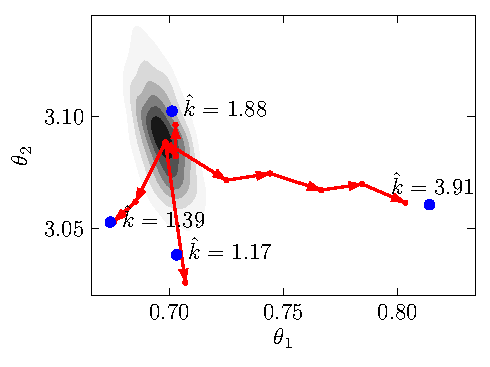
\includegraphics[width = 0.5\textwidth]{figs/illustr_roach2.pdf}
%
\caption{Illustration of the trajectory of the sample mean during the iterative moment matching.
The grey contour lines represent the marginal distribution of
two model parameters in the full data posterior. The blue dots represent
true LOO posterior means corresponding to leaving out influential observations. The red dots represent the means
of the transformed full data posterior draws when iterating the moment matching.} \label{fig:illustr}
\end{figure}






Because the large variance of the importance weights also affects the accuracy
of computing the weighted moments, the moment matching transformations can be noisy.
There are two principal ways to remediate this.
First, increasing the number of draws generally increases accuracy
of the computed moments.
Second, the importance weights used for computing the weighted moments
can be smoothed using Pareto smoothing~\citep{vehtari2017practical}.
We note that using Pareto smoothing for the weighted moments never causes
any bias for the actual estimator that we are interested in, because the importance weights are recomputed after the transformation.
In the experiments section, we demonstrate the performance of the algorithm both with and without Pareto smoothing.



Another shortcoming of the method is that the target distribution is not always well characterized by its first and second moments, and
the target and proposal distributions can differ in several
characteristics, such as tail thickness, correlation structure, or
number of modes.
For complex distributions, more
elaborate transformations may be needed
to reach a good enough proposal distribution.
That being said, it is not necessary to match all characteristics of the
proposal and target distributions for importance sampling to be reliable.











Because the importance weighted moment matching automatically adapts the used proposal
distribution to match the integral being evaluated, it is closely connected to
earlier approaches of adaptive importance sampling~\citep{lepage1978new,ortiz2000adaptive,cappe2004population, pennanen2006adaptive,raftery2010estimating,cornuet2012adaptive}.
Many of these approaches use parametric proposal distributions, and either optimize
the parameters to improve the proposal distribution, or iteratively add more proposal distributions
using multiple importance sampling.
Our approach is independent of the sampling scheme and proposal distribution, and can thus
benefit from efficient MCMC algorithms to sample from complicated
posterior distributions.
Unbiased path sampling by~\citet{rischard2018unbiased} can also use arbitrary proposal distributions, but their approach
requires considerable tuning from the user.





\subsection{Split Transformation Extension for Self-Normalized Importance Sampling} \label{sec:split}






In self-normalized importance sampling, using either the common or the
integrand-specific weights in the moment matching may be beneficial
depending on the situation.
While the moment matching algorithm is designed to decrease the variance
of one type of weights, there is no guarantee as to what happens
to the distribution of the other weights.
For example, if the original proposal distribution is a good candidate for
estimating the numerator in the self-normalized
importance sampling estimator, variance reduction in the common importance weights will likely
increase the variance of the integrand-specific weights. This is exactly what happens
in LOO-CV: Because the integrand-specific weights
all evaluate to one, a successful moment matching transformation using the common weights will \emph{always}
increase the variance of the integrand-specific weights.
A solution that prevents this issue is to
use multiple importance sampling after the moment matching algorithm by
combining the original proposal with the new implicit proposal distribution.
We call this \emph{split moment matching}. It is an extension to the moment matching algorithm, and
can be used after it has completed for small additional computational cost.
The mathematical details of the split moment matching as well as intuition for
its efficacy are discussed in Appendix A.












\subsection{Implementation for LOO-CV}


The moment matching algorithm for LOO-CV is very simple as it does not require
the user to set any parameters, and is thus easily automatized.
We focus on the implementation for the case
of self-normalized importance sampling from the full data posterior
distribution. However, all the basic principles are the same
when sampling from the LOO posterior or when using
an arbitrary proposal distribution.
The benefit of using the full data posterior compared to the LOO posterior
is computational efficiency, as the model has to be fitted only once.
On the other hand, the benefit compared to a simpler parametric proposal distribution
is accuracy: The full data posterior is the optimal proposal distribution
for computing the numerator of the self-normalized importance sampling
estimator, regardless of the model and the shape
of the posterior distribution.



In addition to the log likelihood values for each observation and
each posterior draw that are required by self-normalized importance sampling LOO-CV,
the user must now also provide functions for computing the log posterior density of the model
and the log likelihood based on parameter values in the unconstrained parameter space. The latter is required because moment matching in a constrained space via affine transformations might violate the constraints. Thus, the algorithm operates in the unconstrained space where each parameter can have any real value.
For example, model parameters that are constrained to be positive, can be unconstrained by a log-transformation.



The moment matching algorithm for LOO-CV is as follows:
Using draws from the full data posterior of the model, the algorithm does importance sampling
LOO-CV and computes the Pareto $\hat{k}$ diagnostic for each observation
based on the common importance weights.
Then, moment matching is done for each observation whose Pareto $\hat{k}$ value exceeds
a user-defined threshold value.
For each of those observations, the algorithm iteratively tries one of the three affine transformations
presented in Section~\ref{sec:trans} and recomputes the common importance weights using equation~(\ref{eq:newIR}).
Using again the Pareto diagnostics based on the updated weights, the transformations can be either accepted or rejected
based on whether the diagnostic $\hat{k}$ is decreased or not by the transformation.
%
If the transformation is accepted, the transformed draws are
taken as the new implicit proposal distribution for the particular observation that
is being evaluated, and the importance weights are updated.
This procedure is repeated until none of the three transformations improves the $\hat{k}$ diagnostic value, or
until $\hat{k}$ falls below the user-defined threshold value.
The user can also set a limit for the maximum number of transformations to
perform per observation. If the user chooses, the split transformation
is done when the moment matching is terminated. The final draws and importance weights are used to compute the
updated LOO-CV estimates for the modified LOO folds.
When there are multiple LOO folds with high Pareto $\hat{k}$ values, the moment matching
is embarrassingly parallelizable for the different folds.
The full method is presented as Algorithm~\ref{alg:mm} in Appendix C.


For all LOO folds that are operated on, the Pareto $\hat{k}$ diagnostics
are monitored, and the user is warned if they remain high even after moment matching.
If this happens, refitting the model to the LOO data
and using simple Monte Carlo sampling will often improve
accuracy. If the Pareto $\hat{k}$ diagnostic is still high,
moment matching can be used also with the sample from the LOO posterior.










The moment matching method presented in this work is implemented in R~\citep{rlang}
so that users can easily compare the predictive performance
of models.
The complete code
is available on Github (\url{https://github.com/topipa/iter-mm-paper}).
For importance sampling LOO-CV and the Pareto diagnostics, the method uses
the \texttt{loo} R package~\citep{loo}.
We also provide convenience functions that implement the moment matching method 
for models fitted with probabilistic programming language 
Stan~\citep{carpenter2017stan}. In this case, it is enough that
the user supplies a Stan fit object, where the log likelihood
computation is included in the generated quantities block.
Internally, the method then uses the \texttt{loo} package for importance sampling,
and the given Stan fit object for computing the likelihoods
and posterior densities. Our code is specifically modularized to make it 
straightforward to implement the moment matching also 
for other fitted model objects.








\section{Experiments}





In this section,
the proposed moment matching method is illustrated with six
numerical experiments.
With both simulated and real data sets, we evaluate
the predictive performance of models using self-normalized importance sampling LOO-CV, and demonstrate
the improvements that the moment matching and split moment matching methods can provide.
In addition, we show how simple Monte Carlo sampling from
each LOO posterior performs in comparison.
By default, we use Pareto smoothed importance sampling, both for computing
the LOO-CV estimate and for computing the weighted moments in the moment matching algorithm.
For comparison, we also present results without Pareto smoothing.
In all cases, we monitor the reliability of the Monte Carlo estimates
using the Pareto $\hat{k}$ diagnostics, and show that the
diagnostics accurately identify convergence problems
in all of the used Monte Carlo estimators.
Based on~\citet{vehtari2017practical}, we use $\hat{k} = 0.7$ as
an upper threshold for practically useful convergence rate.


All of the simulations were done in R, and
the models were fitted using \texttt{rstan}, 
the R interface to the Bayesian inference package Stan~\citep{rstan}.
For each model, we ran four chains using a dynamic Hamiltonian Monte Carlo (HMC)
algorithm~\citep{hoffman2014no,Betancourt2017} which is the default in Stan.
%
%
%
We monitor convergence of the chains with the split-$\widehat{R}$ potential scale reduction factor from~\citet{Vehtari+etal:2019:Rhat} and by checking for divergence transitions, which is a diagnostic
specific to adaptive HMC.
%
%
%
%
We note that the finite sample behaviour of Monte Carlo integrals
depends on the algorithm used to generate the sample.
For example, if one uses an MCMC algorithm less efficient than HMC, the
resulting Monte Carlo approximations will generally be even worse than those illustrated in the next sections.
R and Stan codes of the experiments and the used data sets are available on Github (\url{https://github.com/topipa/iter-mm-paper}).






\subsection{Experiment: Toy Example with a Single Outlier} \label{sec:toyexperim}

In this section, we demonstrate with a simple example what happens when
we try to assess the predictive performance of a misspecified model, such that 
there are observations that the model predicts very poorly.
We emphasize that even though this is a simple example, it still provides valuable
insight for real world data and models as
evaluating misspecified models is an integral part of any Bayesian modelling process.





We generate 29 observations from a standard normal distribution, and manually
set the value for a 30th observation in order to represent an outlier.
This mimics a situation where the true data generating mechanism has thicker tails
than the assumed observation model.
Keeping the randomly generated observations fixed, we repeat the experiment
for different values of the outlier ranging from $y_{30} = 0$ to $y_{30} = 12$.
We
model the data with a Gaussian distribution with unknown mean and variance, generate
draws from the model posterior, and evaluate the predictive ability of the model using
LOO-CV.





For all 30 observations represented jointly by the vector $\mathbf{y}$, 
the model is thus
\begin{nalign*}
\mathbf{y} \sim \text{Normal} (\mu,\sigma^2)
\end{nalign*}
with mean $\mu$ and standard deviation $\sigma$. 
We set improper uniform priors on $\mu$ and $\log(\sigma)$.
In this model, the posterior predictive distribution $p (\widetilde{y} | \mathbf{y})$ is known analytically, and is a
$t$-distribution with $n-1$ degrees of freedom, mean at the mean of the data, and
scale $\sqrt{1 + 1/n}$ times the standard deviation of the data, where $n$ is the number of
observations.
Thus, we can compute the Bayesian LOO-CV estimate for the single
left out point analytically via
\begin{nalign*}
\text{elpd}_{\text{loo},i} = \log p (\widetilde{y} = y_i | \mathbf{y}_{-i}).
\end{nalign*}
We then compare the analytical value to different sampling-based estimates:
1) simple Monte Carlo sampling from the LOO posterior (naive);
2) Pareto-smoothed importance sampling from the full data posterior (PSIS);
3) moment matching PSIS (MM-PSIS);
4) split moment matching PSIS (SMM-PSIS).
For all four methods, we generated 4000 posterior draws using Stan.






Figure~\ref{fig:toynormal} shows the computed $\widehat{\text{elpd}}_{\text{loo},i}$ estimates
for the $30$'th observation based on the four sampling methods, which are
compared to the analytical $\text{elpd}_{\text{loo},i}$ values when the outlier
value is varied between 0 and 12.
When the outlier becomes more and more different from the rest of the observations and
the analytical $\text{elpd}_{\text{loo},i}$ decreases, both
the simple Monte Carlo estimate from the true LOO
posterior and the PSIS estimate from the full data posterior
become more and more biased in opposite directions
due to sampling errors.
The moment matching
estimate is often close to the naive sampling estimate, which is an indication that the
moment matching transformation has successfully shifted the sample from the full data posterior close to the
LOO posterior. The split moment matching is the only one
that produces a reliable estimate of the analytical solution.
%The small remaining differences between the naive and MM-PSIS 
%estimates are due to the stopping condition $\hat{k} = 0.5$.
%
%
In Appendix B, we show the results of a similar experiment, where
the randomly generated points $y_{1}$ to $y_{29}$ are re-generated at every repetition
to show that the results are not just specific to this particular data realization.




\begin{figure}[h]
\centering
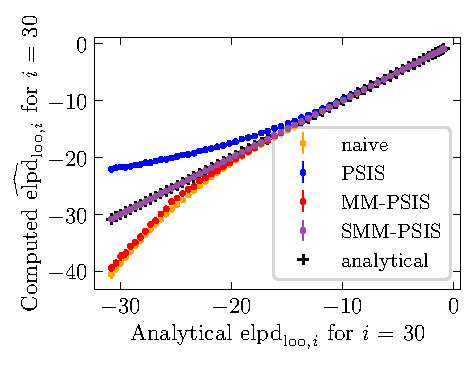
\includegraphics[width=0.5\textwidth]{figs/normaldata_1.pdf}
%
\caption{Computed log predictive density estimates of the left out observation $y_{30}$ for the normal model
for different values between $y_{30} = 0$ and $y_{30} = 12$.
The black line is the analytical LOO predictive density. The sampling results are averaged from 100 independent Stan runs, and the error bars represent $95 \%$
intervals of the mean across these runs.} \label{fig:toynormal}
\end{figure}









In Figure~\ref{fig:normaldata_ks} we show the difference of the computed
$\text{elpd}_{\text{loo},i}$ estimates to the analytical
value together with the diagnostic Pareto $\hat{k}$ values for PSIS, naive and SMM sampling estimates for different values of the outlier. For each sampling method, the
$\hat{k}$ is computed from both the common and integrand-specific weights, and
the larger one is chosen, and
all estimates are averaged from 100 Stan runs.
The figure shows that the Pareto $\hat{k}$ diagnostic value
can diagnose bias in all sampling estimates in a similar manner as long
as both the common and integrand-specific weights are monitored.
A notable difference between the PSIS and naive estimates is the range
that the Pareto $\hat{k}$ takes. This is due to the different nature of the common
and integrand-specific weights, but does not make a difference for
the practical use of the Pareto $\hat{k}$ diagnostic: the threshold
$\hat{k} < 0.7$ indicates practically sufficient rate of convergence in both cases.
We leave further investigation of this phenomenon for future
research.





\begin{figure*}[tbp]
\centering
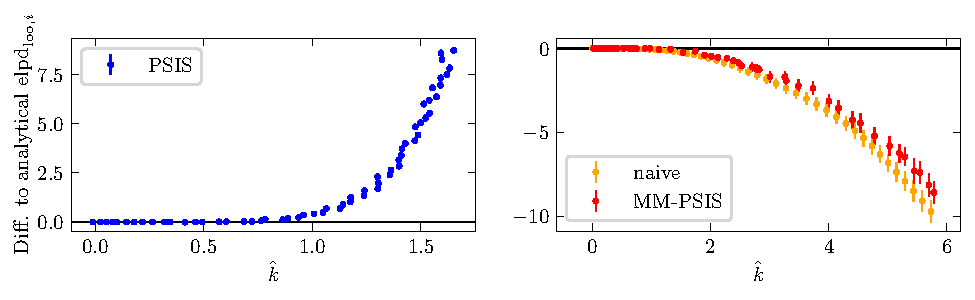
\includegraphics[width=\textwidth]{figs/normaldata_kplots.pdf}
%
\caption{The Pareto $\hat{k}$ diagnostic can reliably diagnose
bias in all sampling estimates. For PSIS, $\hat{k}$ is based on the common importance weights, and
for naive sampling it is based on the integrand-specific weights.
For MM-PSIS, it is the larger of the two $\hat{k}$ estimates.} \label{fig:normaldata_ks}
%
%
\end{figure*}








Figure~\ref{fig:normaldata_x_v_k} shows the importance sampling Pareto $\hat{k}$ values
and naive simple Monte Carlo $\hat{k}$ values as a function of the outlier value $y_{30}$.
Recall that the naive results are fitted to the LOO data where
all observations are from the standard normal distribution.
The figure shows that simple Monte Carlo sampling from the LOO posterior
is more robust to outliers as the
Pareto $\hat{k}$ rises more slowly when increasing the outlier value.
Before exceeding the threshold value $\hat{k} = 0.7$, the outlier can
be about one standard deviation further away compared to importance sampling.
%
%
%
%
%


\begin{figure}[h]
\centering
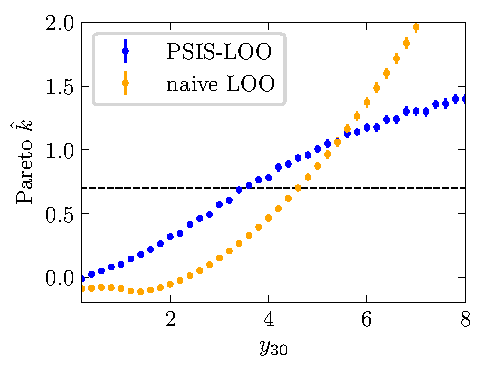
\includegraphics[width=0.5\textwidth]{figs/normaldata_x_v_k.pdf}
%
\caption{Pareto $\hat{k}$ diagnostic values from the common importance weights in
the PSIS estimate and the integrand-specific weights in the naive LOO estimate
for different values of the outlier $y_{30}$.} \label{fig:normaldata_x_v_k}
\end{figure}








Even though this experiment only considered LOO-CV, similar Monte Carlo
sampling errors arise when using independent test data or $k$-fold cross-validation.
For example, if the measured data set included only the randomly generated observations, and the outlier
was part of an independent test set, the log predictive density
estimate would be highly biased similar to the curve in Figure~\ref{fig:toynormal}
corresponding to the naive LOO-CV estimate.








\subsection{Experiment: Poisson Regression with Outliers} \label{sec:poisson}




In the second experiment, we illustrate with a real data set
how unstable Monte Carlo sampling can cause significant errors when estimating predictive performance of models.
The data are from~\citet{gelman2006data}, where the authors describe an experiment that was performed to assess
how efficiently a pest management system reduces the amount of roaches. The target variable $y$ describes the number of roaches
caught in a set of traps in each apartment. The model includes an intercept plus three regression predictors: the number of roaches before treatment, an indicator variable for the treatment or control group, and an indicator variable for whether the building is restricted
to elderly residents.
We will fit a Poisson regression model with a log-link to the data set.
The traps were held in the apartments for different periods of time, so the measurement time is included by adding its logarithm as an offset to the linear predictor.







When fitting the Poisson regression model to the full data set, there are several influential observations that
make estimating the predictive performance of the model with Monte Carlo sampling unrealiable.
In the left side of Figure~\ref{fig:roach_diff} we show the computed $\widehat{\mathrm{elpd}}_{\mathrm{loo}}$
estimates averaged from 100 independent Stan runs as a function of the number of posterior draws $S$.
In the right side, Pareto $\hat{k}$ diagnostic values of 11 influential observations from a single Stan run are shown
for all the methods. The diagnostic is always computed from both
the common and integrand-specific weights, and the larger is reported.
There is a large difference between the PSIS and naive estimates, and they approach each other
very slowly
when increasing $S$, which is due to several LOO folds with high Pareto $\hat{k}$ values.





The moment matching is able to decrease all Pareto $\hat{k}$
values from the common importance weights below $0.7$, and the resulting MM-PSIS estimate is very close
to the naive estimate.
This is because $\hat{k}$
of the integrand-specific weights is increased, as shown in the right plot.
%
The split moment matching can successfully decrease $\hat{k}$ values of the common weights
without consequently increasing $\hat{k}$ of the integrand-specific weights.
This results in accurate $\widehat{\mathrm{elpd}}_{\mathrm{loo}}$ estimates for SMM
that change very little beyond $S = 4000$, whereas the
results of other methods slowly move towards it when increasing the number of posterior draws $S$.
The different sign of the error between the PSIS and naive estimates is a clear indication of a convergence problem
due to not having enough draws from the tails, which results in underestimation
of the evaluated sample mean.
The PSIS estimate is overestimated, because the sample mean
of the common importance weights in the denominator is underestimated.
In Appendix B, we show similar plots that are computed without Pareto smoothing,
and the performance of all methods is essentially the same.





\begin{figure}[h]
\centering
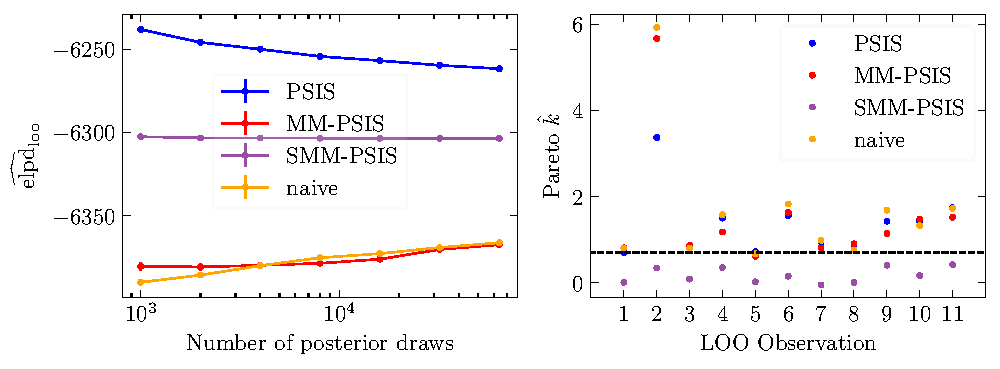
\includegraphics[width=\textwidth]{figs/roach_diff_comb.pdf}
\caption{Left: Computed $\widehat{\mathrm{elpd}}_{\mathrm{loo}}$
estimates as a function of the number of posterior draws $S$
in the roach data set. Right: Pareto $\hat{k}$ diagnostic values for influential observations. The dashed line
at $\hat{k} = 0.7$ indicates the threshold for practically useful convergence rate.} \label{fig:roach_diff}
\end{figure}








\subsection{Experiment: Linear Regression in Stack Loss Data} \label{sec:stackloss}


In this example, we consider the stack loss data set used by~\citet{peruggia1997variability}~and~\citet{vehtari2017practical}. Here, the
distribution of the common importance weights corresponding to the
$21$st observation is known to have infinite variance.
\citet{vehtari2017practical} show that the Pareto $\hat{k}$ diagnostic computed
from a finite set of importance weights is above $0.7$, and the
importance sampling estimate can be biased even with extremely large numbers of
posterior draws.
In the left side of Figure~\ref{fig:stackloss_diff} we show the computed $\widehat{\mathrm{elpd}}_{\mathrm{loo}, i}$
estimates for the $21$st observation as a function of the number of
posterior draws, averaged from 100 independent Stan runs.
In agreement with~\citet{vehtari2017practical},
the PSIS estimate is biased even with more than 100000 draws.
In this case, the naive estimate and the moment matching estimates
are stable from 4000 posterior draws onwards.
In the right side of Figure~\ref{fig:stackloss_diff}, the Pareto
$\hat{k}$ diagnostics averaged from 100 Stan runs are displayed 
with the number of posterior draws, which also indicates that the convergence rate
of naive, MM-PSIS and SMM-PSIS estimates are good, as $\hat{k}$ is significantly below $0.7$.





\begin{figure}[h]
\centering
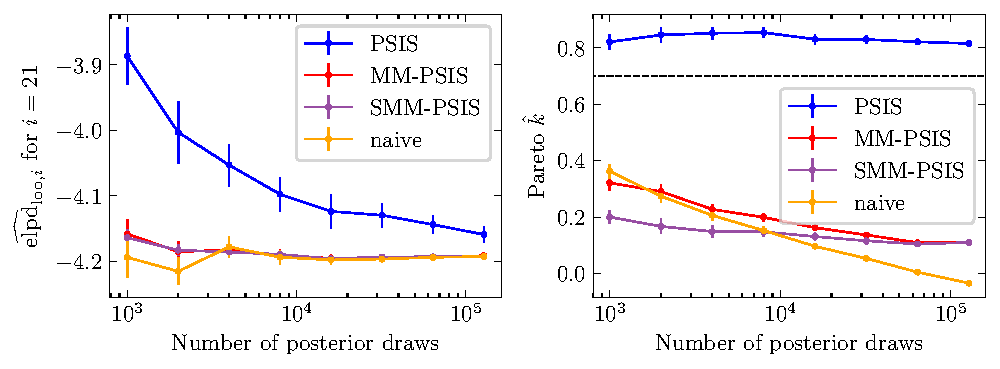
\includegraphics[width=\textwidth]{figs/stackloss_diff_comb.pdf}
\caption{Left: Computed $\widehat{\mathrm{elpd}}_{\mathrm{loo},i}$
estimates for the $21$st observation as a function of the number of posterior draws $S$
in the stack loss data set. The sampling results are averaged from 100 independent Stan runs, and the error bars represent $95 \%$
intervals of the mean across these runs. Right: Pareto $\hat{k}$ diagnostic values of the the $21$st observation with the number of posterior draws $S$. The dashed line
at $\hat{k} = 0.7$ indicates the threshold for practically useful convergence rate.} \label{fig:stackloss_diff}
\end{figure}



This experiment is distinct from Section~\ref{sec:poisson} where
also the naive estimate was significantly biased, which demonstrates the
fact that simple Monte Carlo sampling seems to be more robust to sampling errors
compared to importance sampling.
Thus, in this case, the split moment matching is not strictly necessary, but it does
have smaller variance than the MM estimate or the naive estimate.
In Appendix B, we show similar plots that are computed without Pareto smoothing,
and the performance of all methods is essentially the same.








\subsection{Linear Regression with Correlated Predictor Variables} \label{sec:linreg}



In the previous examples, the used models were quite simple and had a small 
number of parameters. Because of this, the moment matching works almost 
perfectly: It is able to transform the
draws from the full data posterior close to the LOO posteriors and always
reduces the Pareto $\hat{k}$ diagnostic values below $0.7$.
In this and the following sections, we study the limitations of the
moment matching method by considering models with more parameters, correlated
posteriors, and multilevel structures.
For all models, we report the number of LOO folds where
the $\hat{k}$ diagnostic from the common importance weights is above $0.7$, which
is the limit below which practically useful results can be obtained according to~\citet{vehtari2017practical}.
We run the moment matching algorithm for all these LOO folds, and report
how many $\hat{k}$ values are decreased below $0.7$.
Table~\ref{tab:results} shows the number of LOO folds with $\hat{k} > 0.7$
when using PSIS, and after moment matching. The column MM-PSIS corresponds to
moment matching with Pareto smoothed importance weights, and MM-IS
is moment matching without smoothing.



For this experiment,
we simulated data from a linear regression model. 
The data consists of $n = 60$ observations of one outcome variable 
and $30$ predictors that are correlated with each other by correlation coefficient
of $\rho = 0.8$. Three of the true regression coefficients are nonzero, and the rest are all zero. Independent Gaussian noise was added to the outcomes $\mathbf{y}$.
Because the predictors are strongly correlated, importance sampling is
difficult and we get multiple high Pareto $\hat{k}$ values.
%
%
%
%
The results of Table~\ref{tab:results} show that
from 2000 posterior draws onwards, the moment matching algorithm using Pareto smoothing
is able to decrease all Pareto $\hat{k}$ values below $0.7$.
Without Pareto smoothing, moment matching sometimes fails even when
we have a large number of posterior draws.
In Appendix B, we show the results of a similar experiment, where
the data was randomly simulated for each repetition.




\begin{table*}[t]
\centering
\caption{Numbers of LOO folds with Pareto $\hat{k}$ diagnostic above 0.7 when the models are fitted to the full data set. The results are averaged from 100 independent Stan runs. The column MM-PSIS corresponds to
moment matching with Pareto smoothed importance weights, and MM-IS
is moment matching without smoothing.}
\label{tab:results}
\begin{tabular}{ l r r r r }
\hline
Data and model & MCMC Draws & PSIS & MM-PSIS & MM-IS \\
\hline

                      
                      
%
Section~\ref{sec:poisson}: Poisson Regression & $2000$  & 15.2 & 0 & 0  \\
                                   & $4000$  & 14.7 & 0 & 0  \\
                                   & $8000$  & 14.2 & 0 & 0  \\
                                   & $16000$ & 13.2 & 0 & 0  \\
\hline                                    
%
Section~\ref{sec:stackloss}: Linear Regression & $2000$  & 0.8 & 0 & 0  \\
                                       & $4000$  & 0.9 & 0 & 0  \\
                                       & $8000$  & 1.0 & 0 & 0  \\
                                       & $16000$ & 0.9 & 0 & 0  \\
\hline                                    
%
Section~\ref{sec:linreg}: Correlated Predictor Variables       & $2000$  & 14.0 & 0      & 0.6 \\
                                   & $4000$  & 13.8 & 0      & 0.4 \\
                                   & $8000$  & 13.4 & 0      & 0.4 \\
                                   & $16000$ & 12.8 & 0      & 0.2 \\
%
\hline                                    
Section~\ref{sec:ovarian}: Binary Classification $n < p$ & $1000$  & 24.3 & 10.7 & 11.4  \\
                                      & $2000$  & 22.5 & 9.7 & 10.0  \\
                                      & $4000$  & 20.8 & 7.6 & 8.5  \\
                                      & $8000$  & 19.1 & 5.8 & 6.7  \\
\hline                               
%
Section~\ref{sec:radon}: Multilevel Model   & $2000$  & 7.4 & 4.0 & 4.7  \\
                                   & $4000$  & 7.5 & 3.2 & 4.5  \\
                                   & $8000$  & 7.7 & 1.9 & 4.1  \\
                                   & $16000$ & 7.8 & 1.2 & 3.8  \\
                                   & $32000$ & 7.7 & 0.4 & 3.7  \\
\hline
\end{tabular}
\end{table*}







\subsection{Binary Classification in a Small $n$ Large $p$ Data Set} \label{sec:ovarian}

In the fifth experiment, we have a real microarray Ovarian cancer classification data set with a large number of
predictors and small number of observations.
The data set has been used as a benchmark by several authors~(e.g.~\citet{schummer1999comparative,hernandez2010expectation} and references).
The data consists of $54$ measurements and has $1536$ predictor variables.
We will fit a logistic regression model
using a regularized horseshoe prior~\citep{piironen2017rhs} on the regression coefficients because
we expect many of them to be zero.
This data set and model are difficult for several reasons.
Firstly, because of the large number of predictors,
fitting the model takes a long time. Secondly, because
the amount of observations is quite low, many observations are influential
and we get a large number of high Pareto $\hat{k}$
values. Thirdly, because the number of parameters in the model is large,
moment matching in the high-dimensional space is difficult.
Table~\ref{tab:results} shows the number of LOO folds with $\hat{k} > 0.7$
before and after moment matching.
The results show that already with 1000 draws,
many difficult LOO folds can be fixed. Investing more computational resources
by collecting more posterior draws increases
the moment matching accuracy, and more LOO folds can be improved.
However, even with $8000$ posterior draws some folds have $\hat{k} > 0.7$
after moment matching, and thus the $\widehat{\text{elpd}}_{\text{loo}}$
estimate may not be reliable.
In order to decrease each $\hat{k}$ below $0.7$, an impractically large number of
draws might be required.
Thus, it may be necessary to refit the model to the LOO folds
that the moment matching is not able to improve enough.



The used data set and model are complex enough that using brute force LOO-CV takes
a nontrivial amount of time. Omitting parallelization and generating
4000 posterior draws, the model
fit using Stan took an average of 66 minutes. Naive LOO-CV would be costly as fitting the model 54 times would take around 60 hours. 
With the same hardware, standard PSIS took less than a second, but refitting the 20.8 (on average)
problematic LOO folds would take more than 23 hours. At the same time, the (Pareto smoothed) moment matching and split moment matching took a total of only 16 minutes. As the moment matching takes less time than a single refit
while decreasing the number of required refits from 20.8 to 7.6 on average, it
is clearly more computationally efficient.









\subsection{Multilevel Model} \label{sec:radon}


\citet{gelman2006data} describe a study where radon levels were measured in houses
across the United States.
Here, we only consider the measurements from the state of Pennsylvania, from which
there are 2389 observations from 68 different counties. Because the observations have a natural grouping, and
they are distributed unevenly between the counties, we model the radon levels using a multilevel model with varying intercept and varying slope:
\begin{nalign*}
y_i \sim & \; \text{Normal} \left ( \alpha_{j[i]} + \beta_{j[i]} x_i , \sigma^2 \right ) , \\
\alpha_{j[i]} \sim & \; \text{Normal} \left ( \mu_{\alpha} , \sigma_{\alpha}^2 \right ) , \\
\beta_{j[i]} \sim & \; \text{Normal} \left ( \mu_{\beta} , \sigma_{\beta}^2 \right ) ,
\end{nalign*}
where $y_i$ is the logarithm of the radon measurement in the $i$'th house,
$x_i$ is 0 or 1 depending on whether the measurement is from the basement of
the first floor, and $\sigma$ is the standard deviation.
Table~\ref{tab:results} shows the number of LOO folds with $\hat{k} > 0.7$
before and after moment matching.
Again, collecting more posterior draws improves the success rate of moment matching,
and with 32000 draws almost all LOO folds fall below the threshold $\hat{k} = 0.7$.
Without Pareto smoothing, the moment matching requires more draws to reach the same
accuracy.
In this case, it might thus be beneficial to collect enough
draws to get the $\hat{k}$ for all LOO folds below $0.7$, as this
will also increase the Monte Carlo accuracy of all other LOO folds.










\section{Conclusion}

We proposed a method for improving the accuracy
of Monte Carlo approximations to integrals via importance sampling and importance weighted moment matching.
By matching the moments of a Monte Carlo sample to
its importance weighted moments, the proposal
distribution is implicitly modified, improving
the convergence rate of the Monte Carlo estimator.
By differentiating between common and integrand-specific
importance weights, the method is usable in combination with a lot of
different Monte Carlo estimators.
The method is easy to use and automate for different applications because it has
no parameters that require tuning.
We also proposed the split moment matching method, which is an extension that
takes into account the special characteristics of self-normalized importance sampling.




We also generalized the Pareto diagnostic method from~\citet{vehtari2015pareto}
to diagnose inadequate convergence rate for all Monte Carlo estimators, and
demonstrated their usefulness with both self-normalized importance sampling
and simple Monte Carlo sampling. For self-normalized importance sampling, it is essential
to monitor both the common and integrand-specific weights.
We recommend using the proposed diagnostics
whenever computing Monte Carlo approximations to integrals, and
using the moment matching method when the diagnostics indicate inadequate convergence.





We evaluated the efficacy of the proposed methods in self-normalized importance sampling leave-one-out
cross-validation (LOO-CV), and demonstrated that they can often increase the accuracy
of model assessment, and even surpass naive LOO-CV that requires expensive
refitting of the model.
%
%
In models with complex or high-dimensional posterior
distributions, the moment matching is not always successful.
In these cases, the user should
refit the model to the problematic LOO fold, or turn to $k$-fold cross-validation.
In all cases, the convergence diagnostics should be used
to assess the sampling reliability.
We believe that the proposed methods are useful for improving the accuracy of Bayesian model assessment
not only when using cross-validation, but also with independent test data.









\section{Acknowledgements}

We thank M{\aa}ns Magnusson for helpful comments and discussions on earlier versions of this paper.
We also acknowledge the computational resources provided by the Aalto Science-IT project.


%
%
%
\bibliographystyle{apalike}
\bibliography{iter-mm}
%



\onecolumn
\clearpage



\section*{Appendix}






\subsection*{Appendix A: Split Transformation Extension for Self-Normalized Importance Sampling}



The optimal proposal distribution for the self-normalized importance sampling estimator in equation~(\ref{eq:snisopt}) is a piecewise defined function,
%
and can be difficult
to construct in practice.
%
%
However, we can approximate equation~(\ref{eq:snisopt}) with a simpler proposal distribution
superimposed on top of the optimal proposal:
\begin{nalign} \label{eq:5050prop}
g_{\text{split}} (\boldsymbol{\theta}) \propto h(\boldsymbol{\theta}) p (\boldsymbol{\theta})  + \mathbb{E}_p [h(\boldsymbol{\theta})] p (\boldsymbol{\theta}) .
\end{nalign}
Here, $\mathbb{E}_p [h(\boldsymbol{\theta})]$ is the true integral
%
that we are trying to estimate.
This is a convenient approximation to the optimal proposal in equation~(\ref{eq:snisopt}) as it has
similar tails while being simpler to sample from
due to omitting the absolute value.
The drawback of this approximation is that it places unnecessary probability mass in areas where
$h(\boldsymbol{\theta}) \approx \mathbb{E}_p [h(\boldsymbol{\theta})]$, thus losing efficiency.
However, the more distinct $p (\boldsymbol{\theta})$ is from
$p (\boldsymbol{\theta}) |h (\boldsymbol{\theta})|$, the smaller
$\mathbb{E}_p [h(\boldsymbol{\theta})]$ becomes and hence the approximation becomes closer to the optimal form
of equation~(\ref{eq:snisopt}).





If we integrate equation~(\ref{eq:5050prop}) over $\boldsymbol{\theta}$, we notice that
both terms in the sum integrate to $\mathbb{E}_p [h(\boldsymbol{\theta})]$.
Thus, the factor $\mathbb{E}_p [h(\boldsymbol{\theta})]$, even though it is unknown, indicates that both terms in the approximate optimal proposal distribution should
have equal probability mass.
Using this notion, we should aim to construct a multiple importance sampling proposal distribution
consisting of two components that match $p (\boldsymbol{\theta})$ and
$h(\boldsymbol{\theta}) p (\boldsymbol{\theta})$ as closely as possible, and
sample an equal number of draws from both. The restriction is that
we must know the densities of the two components up to the same normalization constant.



By selecting the multiple importance sampling proposals as affine transformed variants
of each other, the difference in normalization constants is known.
Thus, when using the moment matching with self-normalized importance sampling,
we want to find two components that approximate the two components of equation~(\ref{eq:5050prop})
as closely as possible.
If using an arbitrary proposal distribution, one should do two separate moment matching iterations, as
matching the moments to the integrand-specific weights approximates the first component of equation~(\ref{eq:5050prop}), and matching to the common weights approximates the second component.
Denoting $g(\boldsymbol{\theta})$ as our initial proposal distribution, and the implicit
density after an affine transformation $T (\boldsymbol{\theta})$
as $g_T (\boldsymbol{\theta})$, the density of $g_T (\boldsymbol{\theta})$
for any $\boldsymbol{\theta}$ is proportional to the density of $q$ evaluated at $T^{-1} (\boldsymbol{\theta})$.
Denoting the $m$ consecutive transformations with the common weights as $T_w (\boldsymbol{\theta}) = T_{wm} ( ... T_{w2} ( T_{w1} (\boldsymbol{\theta})))$ and the $l$ consecutive transformations with the integrand-specific weights as
$T_{\ome} (\boldsymbol{\theta}) = T_{\ome l} ( ... T_{\ome 2} ( T_{\ome 1} (\boldsymbol{\theta})))$,
a
split proposal density of the form
%\begin{nalign} \label{eq:splitprop-gen}
%g_{\text{split}} (\boldsymbol{\theta}) \propto    g (\boldsymbol{\theta}) + g_T (\boldsymbol{\theta}) \propto    g (\boldsymbol{\theta}) +   |\mathbf{J}_T|^{-1}  g (T^{-1} (\boldsymbol{\theta}))
%\end{nalign}
\begin{nalign} \label{eq:splitprop-gen}
g_{\text{split}} (\boldsymbol{\theta}) \propto    g_{T_w} (\boldsymbol{\theta}) + g_{T_{\ome}} (\boldsymbol{\theta}) \propto    |\mathbf{J}_{T_w}|^{-1}  g ({T_w}^{-1} (\boldsymbol{\theta})) +   |\mathbf{J}_{T_{\ome}}|^{-1}  g ({T_{\ome}}^{-1} (\boldsymbol{\theta}))
\end{nalign}
approximates equation~(\ref{eq:5050prop}) and is usable in self-normalized importance sampling
even if the normalizing constant of $q$ is unknown. The terms
$|\mathbf{J}_{T_i}|^{-1} = \left | \frac{\mathrm{d} {T_i} (\boldsymbol{\theta})}{\mathrm{d} \boldsymbol{\theta}} \right |^{-1}, i = w, \ome $, are the inverses of the Jacobian determinant of the transformations.






In importance sampling LOO-CV, only matching to the common weights is enough, as
the full data posterior $p (\boldsymbol{\theta} | \mathbf{y})$ distribution is already exactly proportional to the first
component of equation~(\ref{eq:5050prop}).
Thus, a moment matched multiple importance sampling proposal distribution for approximating equation~(\ref{eq:5050prop})
is
\begin{nalign} \label{eq:splitprop}
g_{\text{split,LOO}} (\boldsymbol{\theta}) \propto    p (\boldsymbol{\theta} | \mathbf{y})  +  p_{T_w} (\boldsymbol{\theta} | \mathbf{y}) \propto    p (\boldsymbol{\theta} | \mathbf{y})  +   |\mathbf{J}_{T_w}|^{-1}  p ({T_w}^{-1} (\boldsymbol{\theta}) | \mathbf{y}) .
\end{nalign}



When using either equation~(\ref{eq:splitprop-gen})~or~(\ref{eq:splitprop}), half of the
draws should be from the first component and half from the latter.
%The importance weights of the draws based on the mixture proposal in equation~(\ref{eq:splitprop}) are computed as follows.
%First, using draws from the full data posterior, we run the moment matching algorithm normally. After the algorithm has stopped after performing $m$ consecutive transformations, they are combined into a single transformation
%$T (\boldsymbol{\theta}) = T_m ( ... T_2 ( T_1 (\boldsymbol{\theta})))$.
For example, in importance sampling LOO-CV, after performing the moment matching algorithm normally,
the transformations are combined as $T_w (\boldsymbol{\theta}) = T_{wm} ( ... T_{w2} ( T_{w1} (\boldsymbol{\theta})))$, and
only half of the
$S$ of the original draws $\{ \boldsymbol{\theta}^{(s)} \}_{s = 1}^S$ are transformed using $T_w (\boldsymbol{\theta}^{(s)})$:
%
\begin{nalign*}
1 \leq s \leq \frac{S}{2}: \quad  & \transf{\boldsymbol{\theta}}^{(s)}  =  T_w( \boldsymbol{\theta}^{(s)}) \\
\frac{S}{2} < s \leq S: \quad & \transf{\boldsymbol{\theta}}^{(s)}  =  \boldsymbol{\theta}^{(s)} .
\end{nalign*}
We construct analogically an inverse transformation $T_w^{-1} (\boldsymbol{\theta}) = T_{w1}^{-1} ( T_{w2}^{-1} ... ( T_{wm}^{-1} (\boldsymbol{\theta})))$ and a pseudo-set of draws as $\transf{\boldsymbol{\theta}}^{(s)}_{\text{inv}} = T_w^{-1} (\transf{\boldsymbol{\theta}}^{(s)})$, i.e.
\begin{nalign*}
1 \leq s \leq \frac{S}{2}: \quad  & \transf{\boldsymbol{\theta}}^{(s)}_{\text{inv}}  =   \boldsymbol{\theta}^{(s)} \\
\frac{S}{2} < s \leq S: \quad & \transf{\boldsymbol{\theta}}^{(s)}_{\text{inv}}  = T_w^{-1} ( \boldsymbol{\theta}^{(s)} ).
\end{nalign*}
%
Then, the importance weights are computed as
\begin{nalign*}
\widetilde{\transf{w}}_{\text{loo, split},i}^{(s)} = & \frac{p(\transf{\boldsymbol{\theta}}^{(s)}|\mathbf{y}_{-i})} {     g_{\text{split}} (\transf{\boldsymbol{\theta}}^{(s)})  }
 = \frac{p(\transf{\boldsymbol{\theta}}^{(s)}|\mathbf{y}_{-i})} {    p(\transf{\boldsymbol{\theta}}^{(s)}|\mathbf{y}) + |\mathbf{J}_{T_w}|^{-1} p( T_w^{-1} (\transf{\boldsymbol{\theta}}^{(s)}) |\mathbf{y})  } 
= & \frac{p(\transf{\boldsymbol{\theta}}^{(s)}|\mathbf{y}_{-i})} {    p(\transf{\boldsymbol{\theta}}^{(s)}|\mathbf{y}) + |\mathbf{J}_{T_w}|^{-1} p( \transf{\boldsymbol{\theta}}_{\text{inv}}^{(s)} |\mathbf{y})  } \\
= & \frac{p(\transf{\boldsymbol{\theta}}^{(s)}|\mathbf{y})} { p(y_i | \transf{\boldsymbol{\theta}}^{(s)}) [   p(\transf{\boldsymbol{\theta}}^{(s)}|\mathbf{y}) + |\mathbf{J}_{T_w}|^{-1} p( \transf{\boldsymbol{\theta}}_{\text{inv}}^{(s)} |\mathbf{y}) ] } .
\end{nalign*}







\subsection*{Appendix B: Additional Results}






\subsubsection*{Normal Model: Optimality of the Split Proposal Distribution}


For illustrationary purposes, let us simplify the normal model from Section~\ref{sec:toyexperim} such that we assume the variance
of the normally distributed data is known. Then, the model has just one parameter, the mean
of the data, and the posterior distribution
of that parameter is Gaussian.
Using the one-dimensional posterior, we can efficiently visualize
why both the LOO posterior and the full data posterior can
be inadequate proposal distributions for self-normalized importance sampling LOO-CV.
In the top row of Figure~\ref{fig:optimal_vs_smm_3} we illustrate
the LOO posterior and the full data posterior of the model together with
the optimal proposal distribution for computing the self-normalized
importance sampling LOO-CV estimate when we move the outlier $y_{30}$ further. It is evident that
when the left-out observation is influential,
neither the LOO posterior nor the full data posterior can
provide enough draws from one of the tails to adequately estimate the LOO-CV integral.
In the bottom row of Figure~\ref{fig:optimal_vs_smm_3} we illustrate the split proposal distribution in equation~(\ref{eq:5050prop}), which
conversely becomes closer and closer to the optimal proposal distribution
when the left-out observation $y_{30}$ becomes more anomalous.






\begin{figure}[h]
\centering
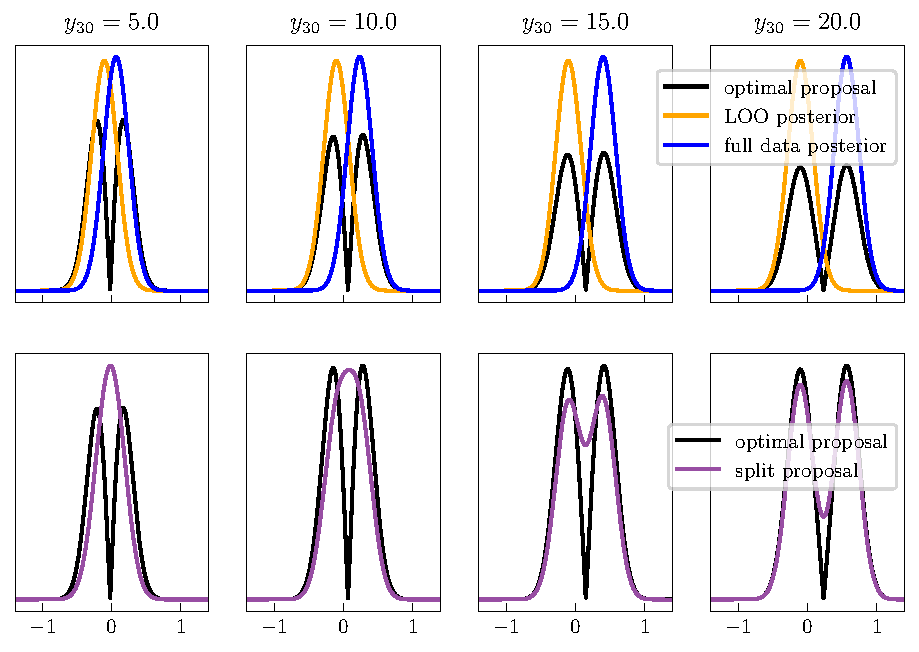
\includegraphics[]{figs/normalmodel_optimal_prop.pdf}
\caption{For the normal model with known variance, the shape of
the optimal proposal distribution together with different proposal distributions
for different values of the outlier $y_{30}$.
Top row: LOO posterior and full data posterior.
Bottom row: Split proposal distribution from equation~(\ref{eq:5050prop}).} \label{fig:optimal_vs_smm_3}
\end{figure}







\subsubsection*{Normal Model: Randomly Generated Data}

In Figure~\ref{fig:toynormal_randomized}, the results of Figure~\ref{fig:toynormal}
are replicated, but now the normally distributed observations $y_{1}$ to $y_{29}$
are different for each Stan run. The results are in principle similar:
All estimates except SMM-PSIS become biased as the outlier moves further.


\begin{figure}[h]
\centering
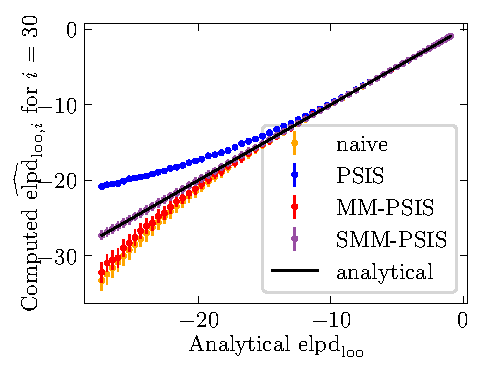
\includegraphics[width=0.5\textwidth]{figs/normaldata_1_randomized.pdf}
%
\caption{Computed log predictive density estimates of the left out observation $y_{30}$
for different values between $y_{30} = 0$ and $y_{30} = 12$ in the Gaussian model of Section~\ref{sec:toyexperim}.
The black line is the analytical LOO predictive density. The sampling results are averaged from 100 independent Stan runs, and the error bars represent $95 \%$
intervals of the mean across these runs. For every Stan run, the observations $y_{1}$ to $y_{29}$
are randomly re-generated.} \label{fig:toynormal_randomized}
\end{figure}










\subsubsection*{Poisson Regression Model: Moment Matching Without Pareto Smoothing}


In Figure~\ref{fig:roach_diff2} we show the computed $\widehat{\mathrm{elpd}}_{\mathrm{loo}}$
estimates averaged from 100 independent Stan runs as a function of the number of posterior draws $S$
in the Poisson regression example.
The figure is similar to Figure~\ref{fig:roach_diff}, but the
estimates are computed without Pareto smoothing.



\begin{figure}[h]
\centering
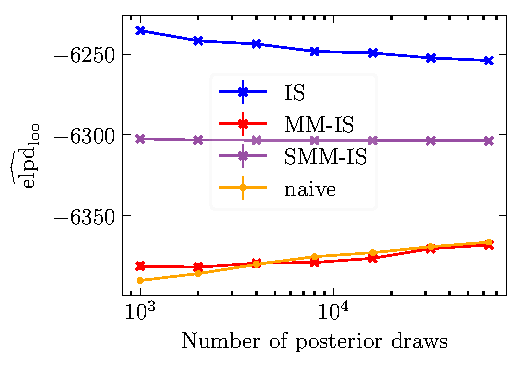
\includegraphics[width=0.5\textwidth]{figs/roach_diff2.pdf}
\caption{Computed $\widehat{\mathrm{elpd}}_{\mathrm{loo}}$
estimates as a function of the number of posterior draws $S$
in the roach data set.} \label{fig:roach_diff2}
\end{figure}




\subsubsection*{Stack Loss: Moment Matching Without Pareto Smoothing}



In Figure~\ref{fig:stackloss_diff2} we show the computed $\widehat{\mathrm{elpd}}_{\mathrm{loo}}$
estimates averaged from 100 independent Stan runs as a function of the number of posterior draws $S$
in the Stack loss example.
The figure is similar to Figure~\ref{fig:stackloss_diff}, but the
estimates are computed without Pareto smoothing.


\begin{figure}[h]
\centering
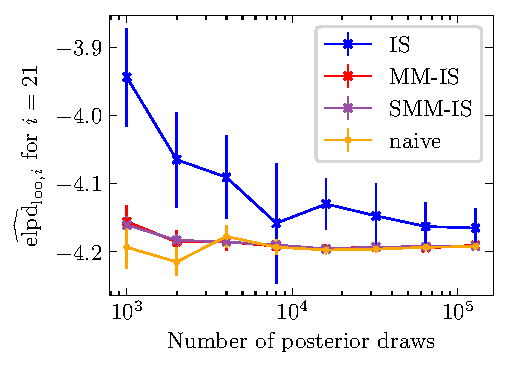
\includegraphics[width=0.5\textwidth]{figs/stackloss_diff2.pdf}
\caption{Computed $\widehat{\mathrm{elpd}}_{\mathrm{loo},i}$
estimates for the $21$st observation as a function of the number of posterior draws $S$
in the stack loss data set.} \label{fig:stackloss_diff2}
\end{figure}















\subsubsection*{Correlated Linear Regression: Different Data Sets}

For the linear regression example in Section~\ref{sec:linreg},
Table~\ref{tab:results_randomized} shows the number of LOO folds with $\hat{k} > 0.7$
before and after moment matching both with and without Pareto smoothing for the weighted moments. The difference to
Table~\ref{tab:results} is that here the data set in randomly
generated for each Stan repetition.


\begin{table*}[t]
\centering
\begin{tabular}{ l r r r r }
\hline
Data and model & MCMC Draws & PSIS & MM-PSIS & MM-IS \\
\hline


Correlated linear regression       & $2000$  & 13.8 & 0      & 0.5 \\
                                   & $4000$  & 13.2 & 0      & 0.3 \\
                                   & $8000$  & 13.0 & 0      & 0.2 \\
                                   & $16000$ & 12.0 & 0      & 0.1 \\
\hline
\end{tabular}
\caption{Numbers of LOO folds with Pareto $\hat{k}$ estimate above 0.7. The results are averaged from 100 independent Stan runs, where the data is re-generated for each repetition.}
\label{tab:results_randomized}
\end{table*}











\subsection*{Appendix C: Iterative moment matching algorithm for LOO-CV}





\begin{algorithm*}[htb]
	\caption{\em Iterative moment matching LOO-CV}\label{alg:mm}
	\begin{algorithmic}[1]
	    \STATE Define stopping threshold $k_{\text{threshold}}$ corresponding to Pareto $\hat{k}$
	    diagnostic value;
		%
		\STATE Run inference to obtain a sample $\{ \boldsymbol{\theta}^{(s)} \}_{s = 1}^S$ from the full data posterior of the model $\widetilde{p} (\boldsymbol{\theta} | \mathbf{y})$;
		\STATE For each draw $\boldsymbol{\theta}^{(s)}$, precompute the full data posterior density $Q_s = \widetilde{p} (\boldsymbol{\theta}^{(s)}|\mathbf{y})$
		 
		\FOR{observation $i$ in $1:n$}
		\STATE Initialize draws for this LOO fold as $\{ \boldsymbol{\theta}_i^{(s)} \}_{s = 1}^S = \{ \boldsymbol{\theta}^{(s)} \}_{s = 1}^S$;
		\STATE Compute common importance weights $\widetilde{w}_{\text{loo},i}^{(s)} = p (y_i | \boldsymbol{\theta}^{(s)})^{-1}$;
		\STATE Fit generalized Pareto distribution to the largest weights $\widetilde{w}_{\text{loo},i}^{(s)}$ and report the shape parameter $\hat{k}_i$;
		\IF{   $\hat{k}_i < k_{\text{threshold}}$  }
		\STATE Compute the estimate $\widehat{\text{elpd}}_{\text{loo},i}$ using Pareto smoothed self-normalized importance sampling;
		\ELSE
		
		\STATE Run \textbf{Algorithm 2}: Moment matching for self-normalized importance sampling;

		\IF{   $\hat{k}_i < k_{\text{threshold}}$  }
		\STATE Compute the estimate $\widehat{\text{elpd}}_{\text{loo},i}$ using Pareto smoothed self-normalized importance sampling;
		\ELSE
		\STATE Run inference to obtain a sample $\{ \boldsymbol{\theta}_i^{(s)} \}_{s = 1}^S$ from the LOO posterior $\widetilde{p} (\boldsymbol{\theta} | \mathbf{y}_{-i})$;
		\STATE Fit generalized Pareto distribution to the largest integrand-specific weights
		$\widetilde{\ome}_{\text{loo},i}^{(s)} = p(y_i | \boldsymbol{\theta}^{(s)})$ and report the shape parameter $\hat{k}_i$;
		\IF{   $\hat{k}_i < k_{\text{threshold}}$  }
		\STATE Compute the estimate $\widehat{\text{elpd}}_{\text{loo},i}$ using simple Monte Carlo sampling;
		\ELSE
		
		
		
		\STATE Run \textbf{Algorithm 3}: Moment matching for simple Monte Carlo sampling;
		

		
		
		
		\ENDIF
		\ENDIF
		\ENDIF
		\ENDFOR
		 
	\end{algorithmic}
\end{algorithm*}






\begin{algorithm*}[htb]
	\caption{\em Moment matching for self-normalized importance sampling}\label{alg:mm-psis}
	\begin{algorithmic}[1]
	\STATE Define the affine transformations $T_1 , ... , T_{n_{\text{trans}}}$;
	\WHILE{$\hat{k}_i > k_{\text{threshold}}$}
	    \FOR{$j$ in $1:n_{\text{trans}}$}
		
		%
		%
		\STATE Transform the draws: $T_J: \boldsymbol{\theta}_i^{(s)} \mapsto \transf{\boldsymbol{\theta}}_i^{(s)}$;
		\STATE Recompute common importance weights $\widetilde{\transf{w}}_{\text{loo},i}^{(s)} = \widetilde{p} (\transf{\boldsymbol{\theta}}^{(s)}|\mathbf{y})/[Q_s p(y_{i}|\transf{\boldsymbol{\theta}}^{(s)})]$;
		\STATE Fit generalized Pareto distribution to the largest common importance weights $\widetilde{\transf{w}}_{\text{loo},i}^{(s)}$ and report the shape parameter $\hat{\transf{k}}_i$;
		\IF{$\hat{\transf{k}}_i < \hat{k}_i$}
		\STATE Accept the transformation and update $\{ \boldsymbol{\theta}_i^{(s)} \}_{s = 1}^S = \{ \transf{\boldsymbol{\theta}}_i^{(s)} \}_{s = 1}^S$, $\{ \widetilde{w}_{\text{loo},i}^{(s)} \}_{s = 1}^S = \{ \widetilde{\transf{w}}_{\text{loo},i}^{(s)} \}_{s = 1}^S$, and $\hat{k}_i = \hat{\transf{k}}_i$;
		\STATE Return to check the while condition;
		\ELSE
		\STATE Discard the transformation;
		\ENDIF
		
		
		\ENDFOR
		
		\IF{$j == n_{\text{trans}}$}
		\STATE Moment matching failed, exit while loop;
		\ENDIF
		
		\ENDWHILE
		 
	\end{algorithmic}
\end{algorithm*}





\begin{algorithm*}[htb]
	\caption{\em Moment matching for simple Monte Carlo sampling}\label{alg:mm-smc}
	\begin{algorithmic}[1]
	\STATE Define the affine transformations $T_1 , ... , T_{n_{\text{trans}}}$;
	    \STATE For each draw $\boldsymbol{\theta}^{(s)}$, precompute the LOO posterior density $Q_s = \widetilde{p} (\boldsymbol{\theta}^{(s)}|\mathbf{y}_{-i})$
	    
	    \WHILE{$\hat{k}_i > k_{\text{threshold}}$}
	    \FOR{$j$ in $1:n_{\text{trans}}$}
		
		%
		%
		\STATE Transform the draws: $T_J: \boldsymbol{\theta}_i^{(s)} \mapsto \transf{\boldsymbol{\theta}}_i^{(s)}$;
		\STATE Recompute importance weights $\widetilde{\transf{w}}_{\text{loo},i}^{(s)} = \widetilde{p} (\transf{\boldsymbol{\theta}}^{(s)}|\mathbf{y}_{-i}) |\mathbf{J}_T| /Q_s$ and integrand-specific weights
		$\widetilde{\transf{\ome}}_{\text{loo},i}^{(s)} = \widetilde{\transf{w}}_{\text{loo},i}^{(s)} \; p(y_i | \boldsymbol{\theta}^{(s)})$;
		\STATE Fit generalized Pareto distribution to the largest integrand-specific importance weights $\widetilde{\transf{\ome}}_{\text{loo},i}^{(s)}$ and report the shape parameter $\hat{\transf{k}}_i$;
		\IF{$\hat{\transf{k}}_i < \hat{k}_i$}
		\STATE Accept the transformation and update $\{ \boldsymbol{\theta}_i^{(s)} \}_{s = 1}^S = \{ \transf{\boldsymbol{\theta}}_i^{(s)} \}_{s = 1}^S$, $\{ \widetilde{w}_{\text{loo},i}^{(s)} \}_{s = 1}^S = \{ \widetilde{\transf{w}}_{\text{loo},i}^{(s)} \}_{s = 1}^S$, and $\hat{k}_i = \hat{\transf{k}}_i$;
		\STATE Return to check the while condition;
		\ELSE
		\STATE Discard the transformation;
		\ENDIF
		
		
		\ENDFOR
		
		\IF{$j == n_{\text{trans}}$}
		\STATE Moment matching failed, exit while loop;
		\ENDIF
		
		\ENDWHILE
		 
	\end{algorithmic}
\end{algorithm*}











\end{document}
